\documentclass{beamer}
\usepackage{gillius}

\usetheme[everytitleformat=regular]{m}
\setbeamertemplate{navigation symbols}{}

\title{How the dynamics and structure of sexual contact networks shape pathogen
       phylogenies}
\author[Robinson et al.]{Katy Robinson \and Nick Fyson \and Ted Cohen \and
Christophe Fraser \and Caroline Colijn}

\begin{document}
\definecolor{red}{RGB}{228,26,28}
\definecolor{blue}{RGB}{55,126,184}
\definecolor{green}{RGB}{77,175,74}
\definecolor{purple}{RGB}{152,78,163}

\maketitle

\begin{frame}{Motivation}
    \begin{itemize}
        \item Information about contact networks is highly useful but
            challenging to gather.
        \item Contact networks affect the shape of pathogen phylogenies.
        \item Is there anything phylogenies can tell us that public health
            monitoring can't?
    \end{itemize}
    \begin{center}
        \itshape
        Here we ask to what extent dynamic host contact networks shape pathogen
        phylogenies, under conditions when the epidemic has similar
        trajectories on different networks.
        \normalfont
    \end{center}
\end{frame}

\begin{frame}{How phylogenies are shaped}
    \vspace{-0.5cm}
    \begin{center}
        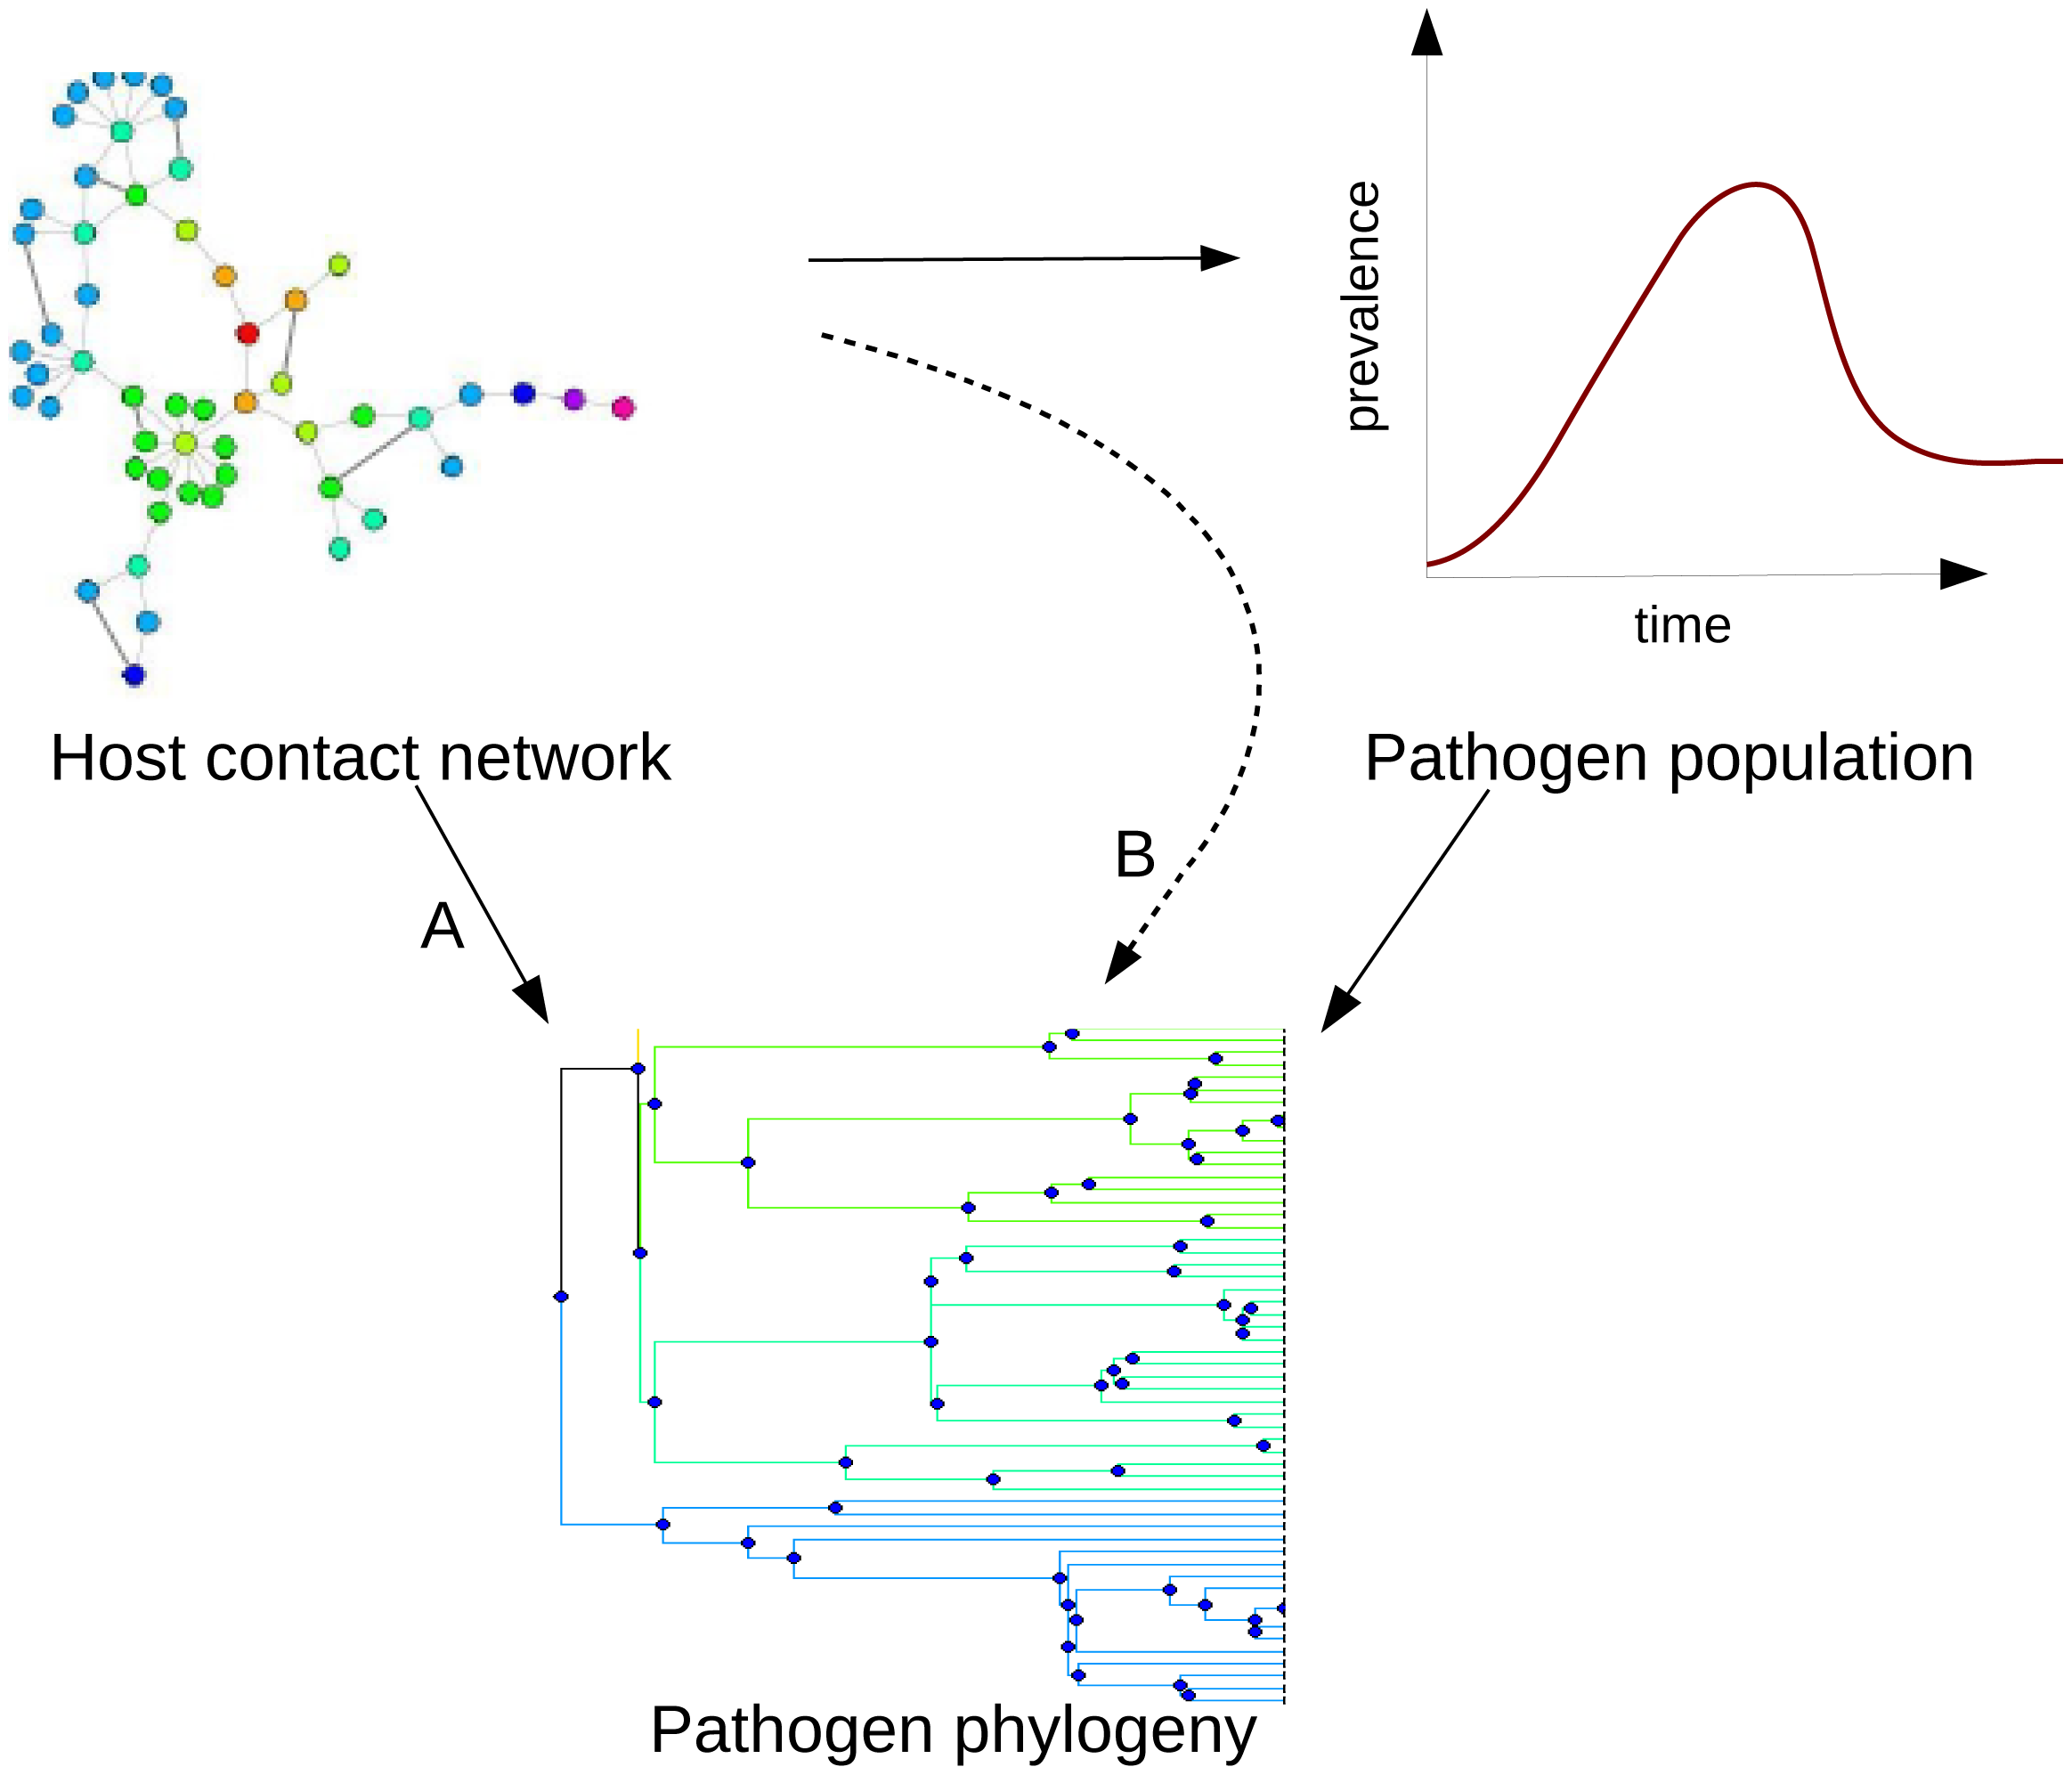
\includegraphics[height=0.8\textheight]{f1}
    \end{center}
\end{frame}

\begin{frame}{Methods: simulations}
    \begin{itemize}
        \item Two types of dynamic network.
            \begin{itemize}
                \item Degree distribution from the British National Survey of
                    Sexual Attitudes and Lifestyles (NATSAL).
                \item Random.
            \end{itemize}
        \item Pathogens with 10- and 40-week durations of infectiousness.
        \item Simulated transmission and sequence evolution over the network.
            \begin{itemize}
                \item Transmission and mutation are both Poisson processes.
                \item One sequence per patient; no selection.
                \item When did they stop the simulation?
            \end{itemize}
    \end{itemize}
\end{frame}

\begin{frame}{Methods: phylogenetics}
    \begin{itemize}
        \item Three sampling schemes.
            \begin{itemize}
                \item 100 sequences at 2 time points.
                \item Uniform number of samples over time.
                \item Proportional sampling over time.
            \end{itemize}
        \item Maximum likelihood phylogenies with PHYLIP.
        \item Clustering by genetic distance cutoff (0.06 expected
            substitutions per site).
        \item Colless' index:
            \[
                \frac{2}{(n-1)(n-2)} \sum_b \lVert T_{iR} - T_{iL} \rVert.
            \]
    \end{itemize}
\end{frame}

\begin{frame}{Results: tree shapes}
    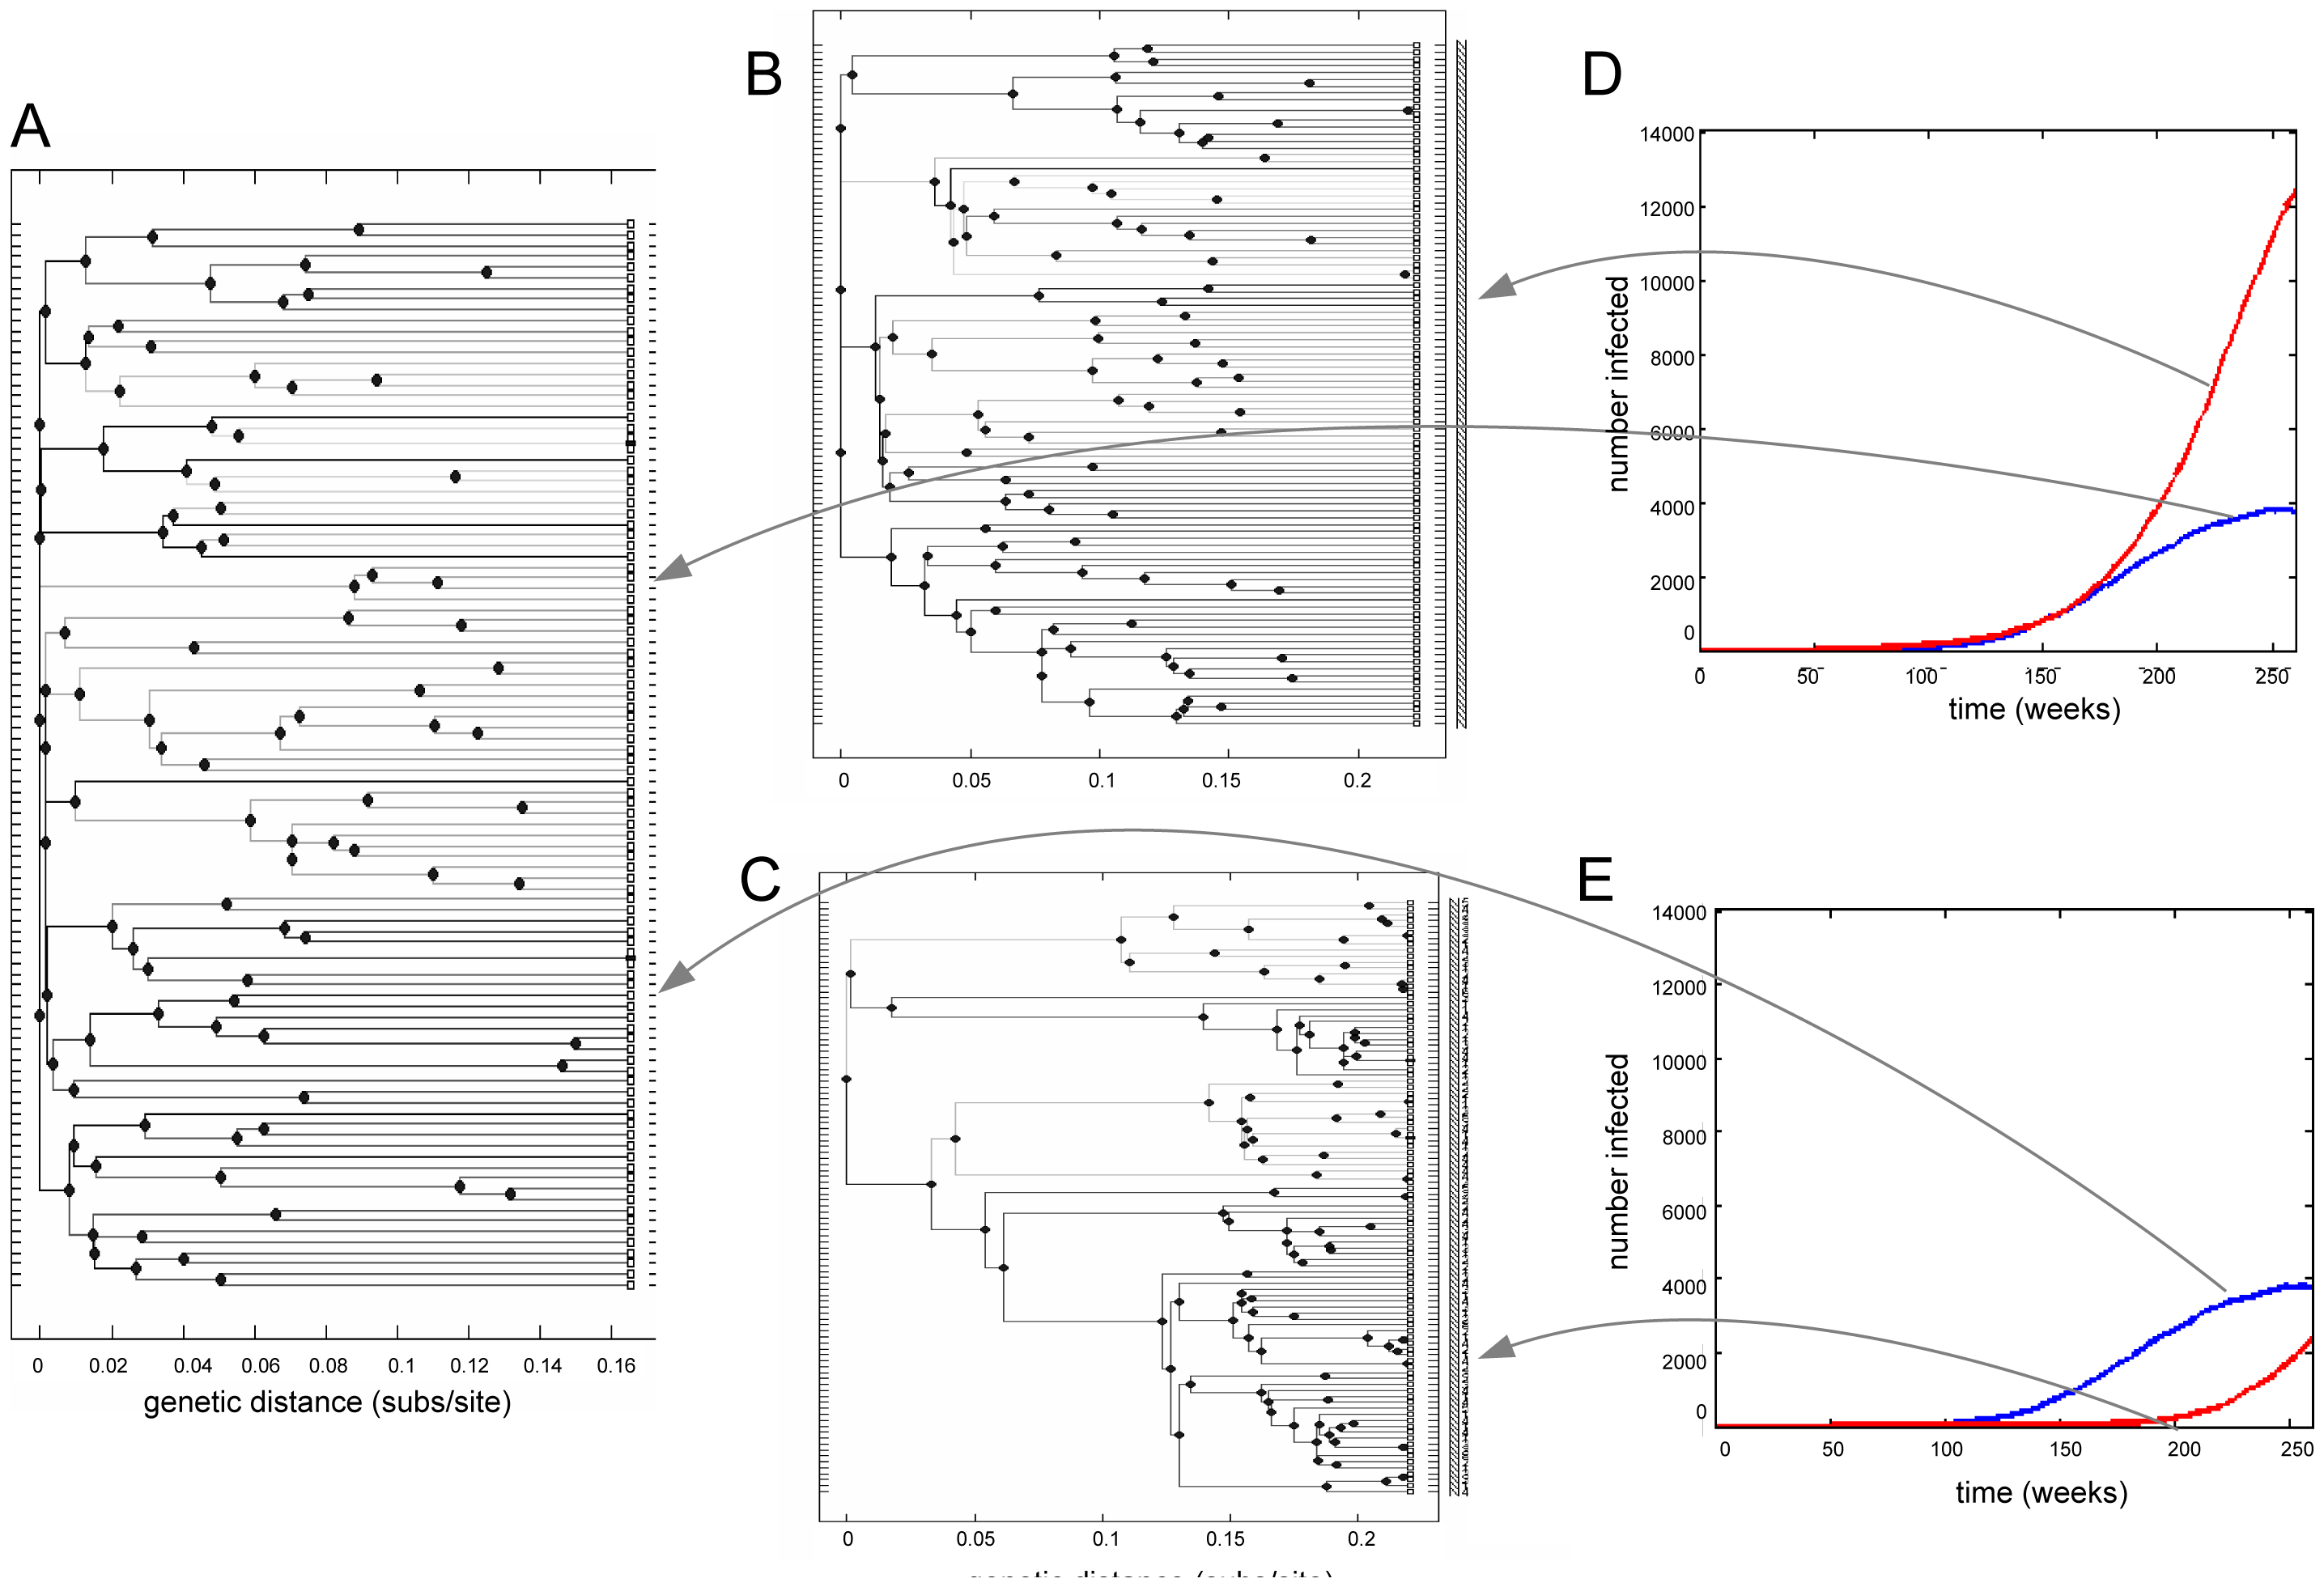
\includegraphics[width=\textwidth]{f2}
\end{frame}

\begin{frame}{Results: cluster numbers and sizes}
    \begin{center}
        \vspace{-0.5cm}
        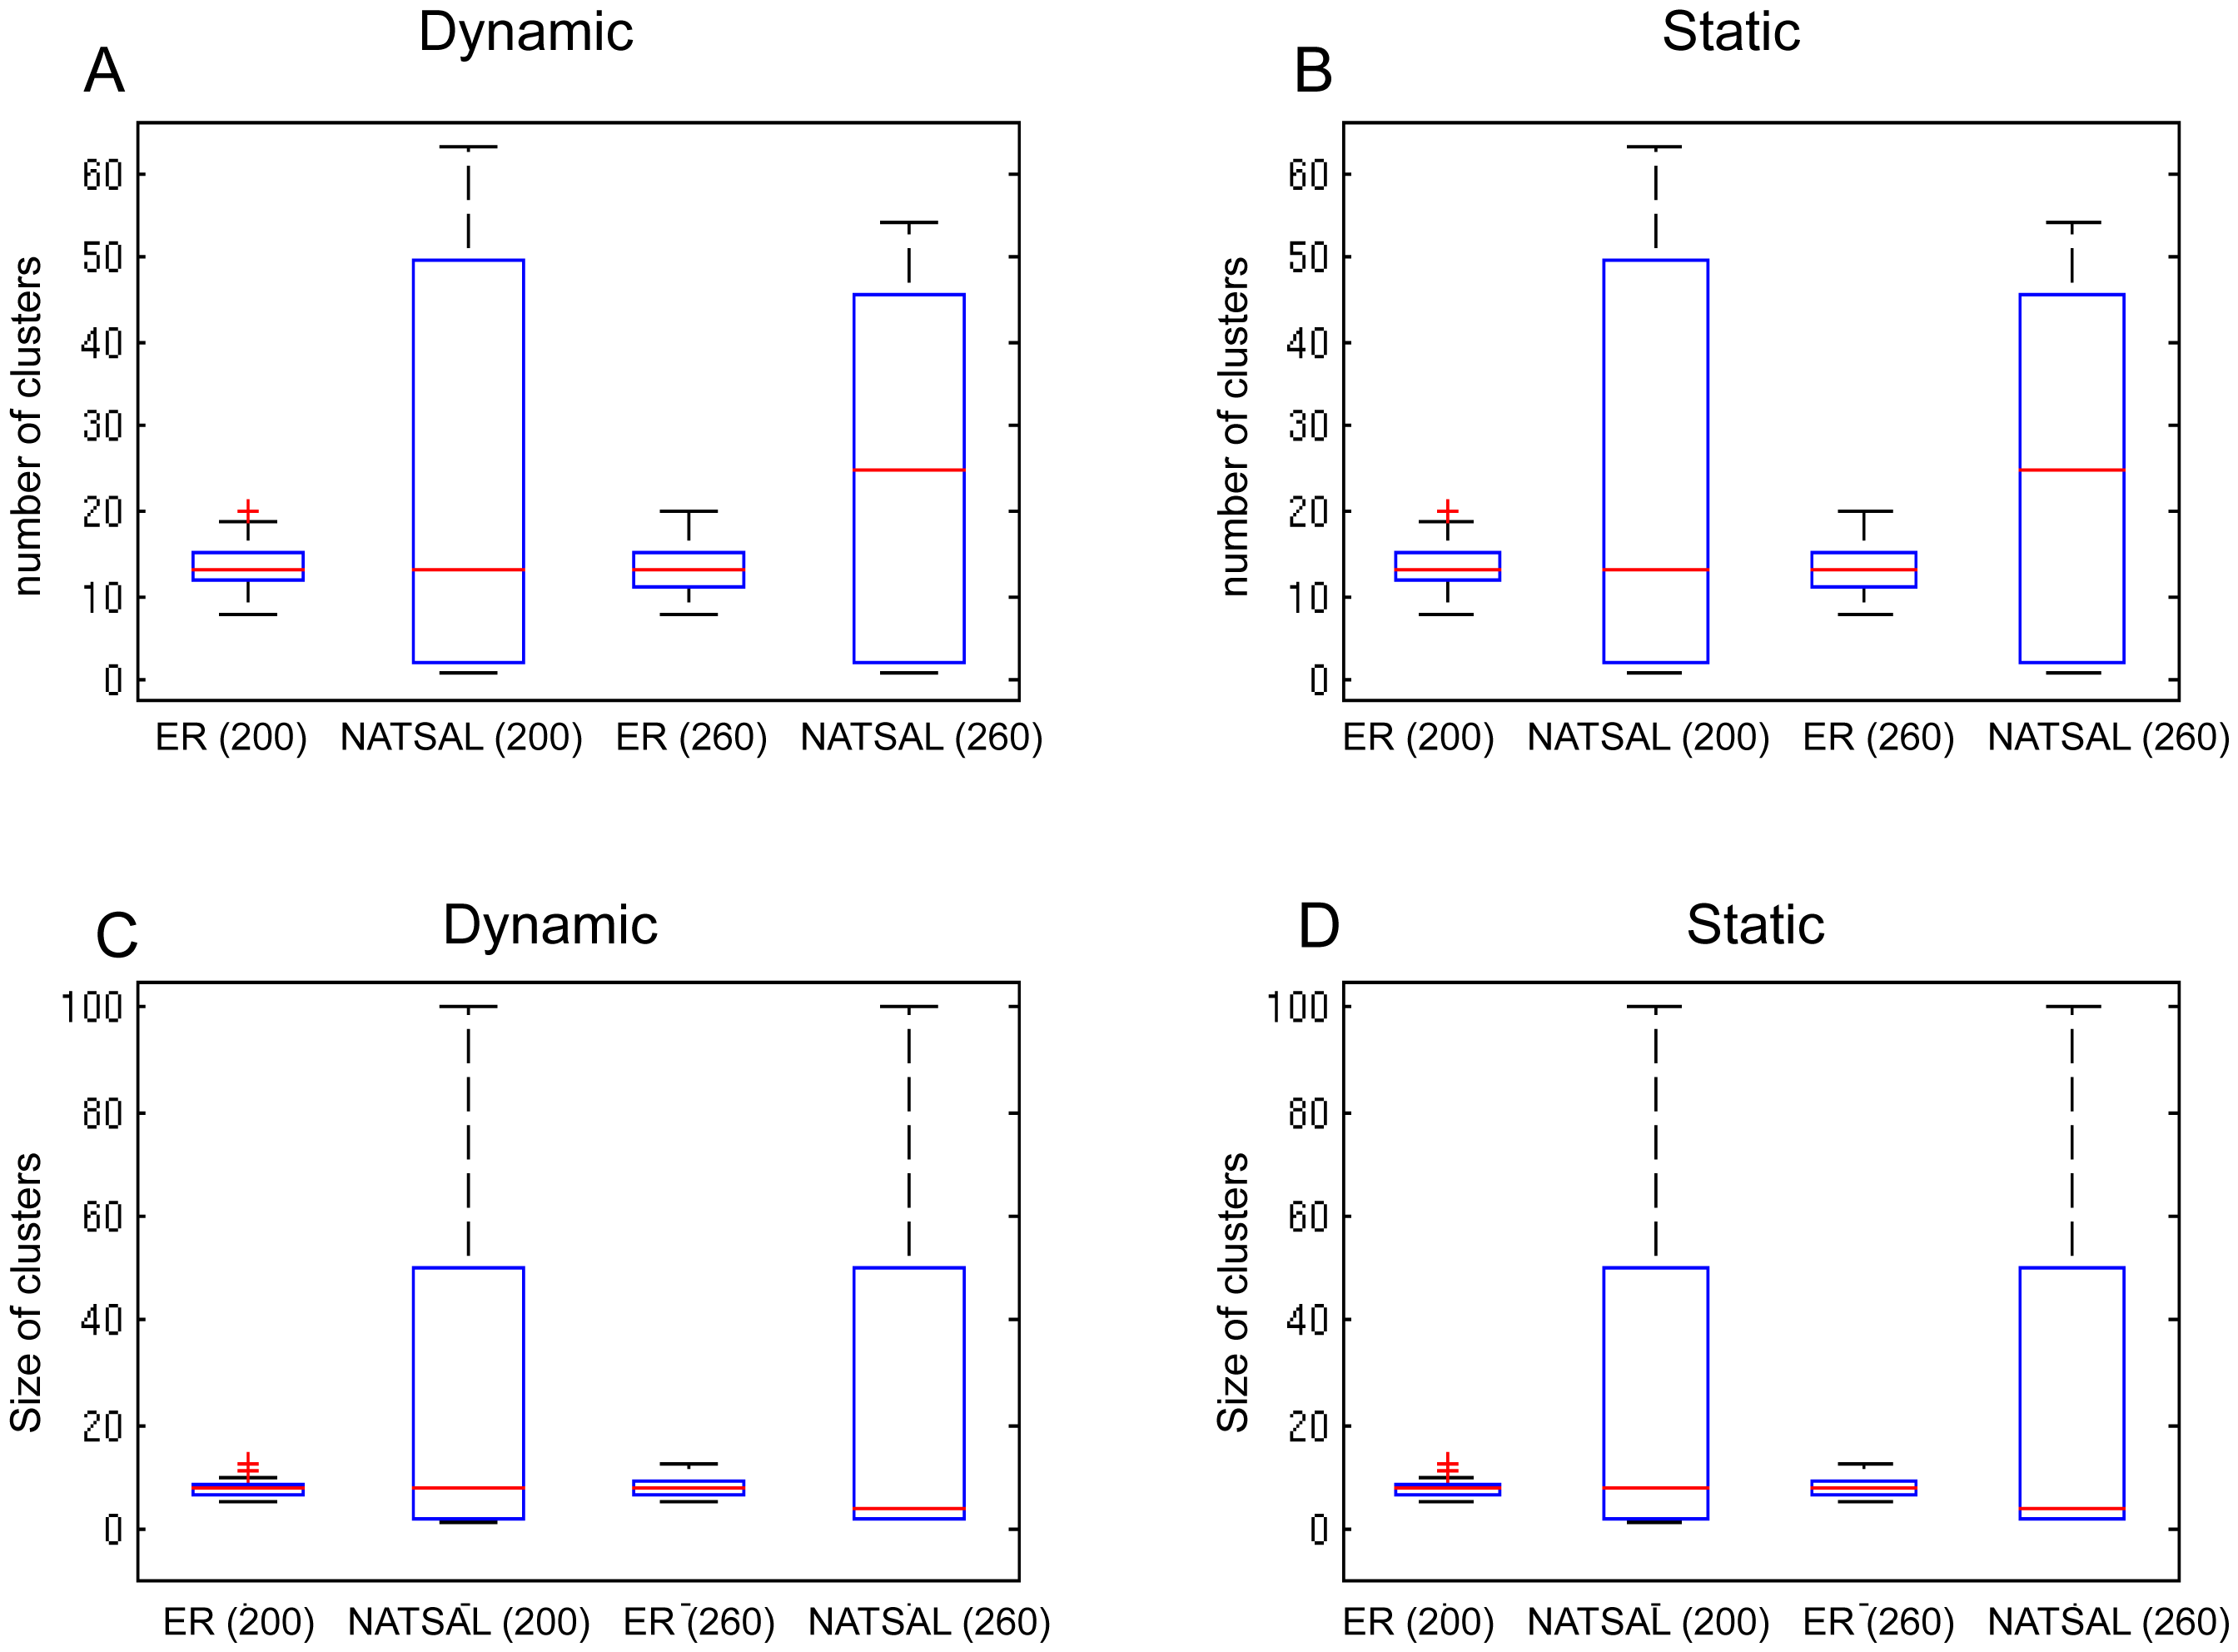
\includegraphics[width=0.9\textwidth]{f3}
    \end{center}
\end{frame}

\begin{frame}{Results: network influences tree size}
    \begin{center}
        \vspace{-0.5cm}
        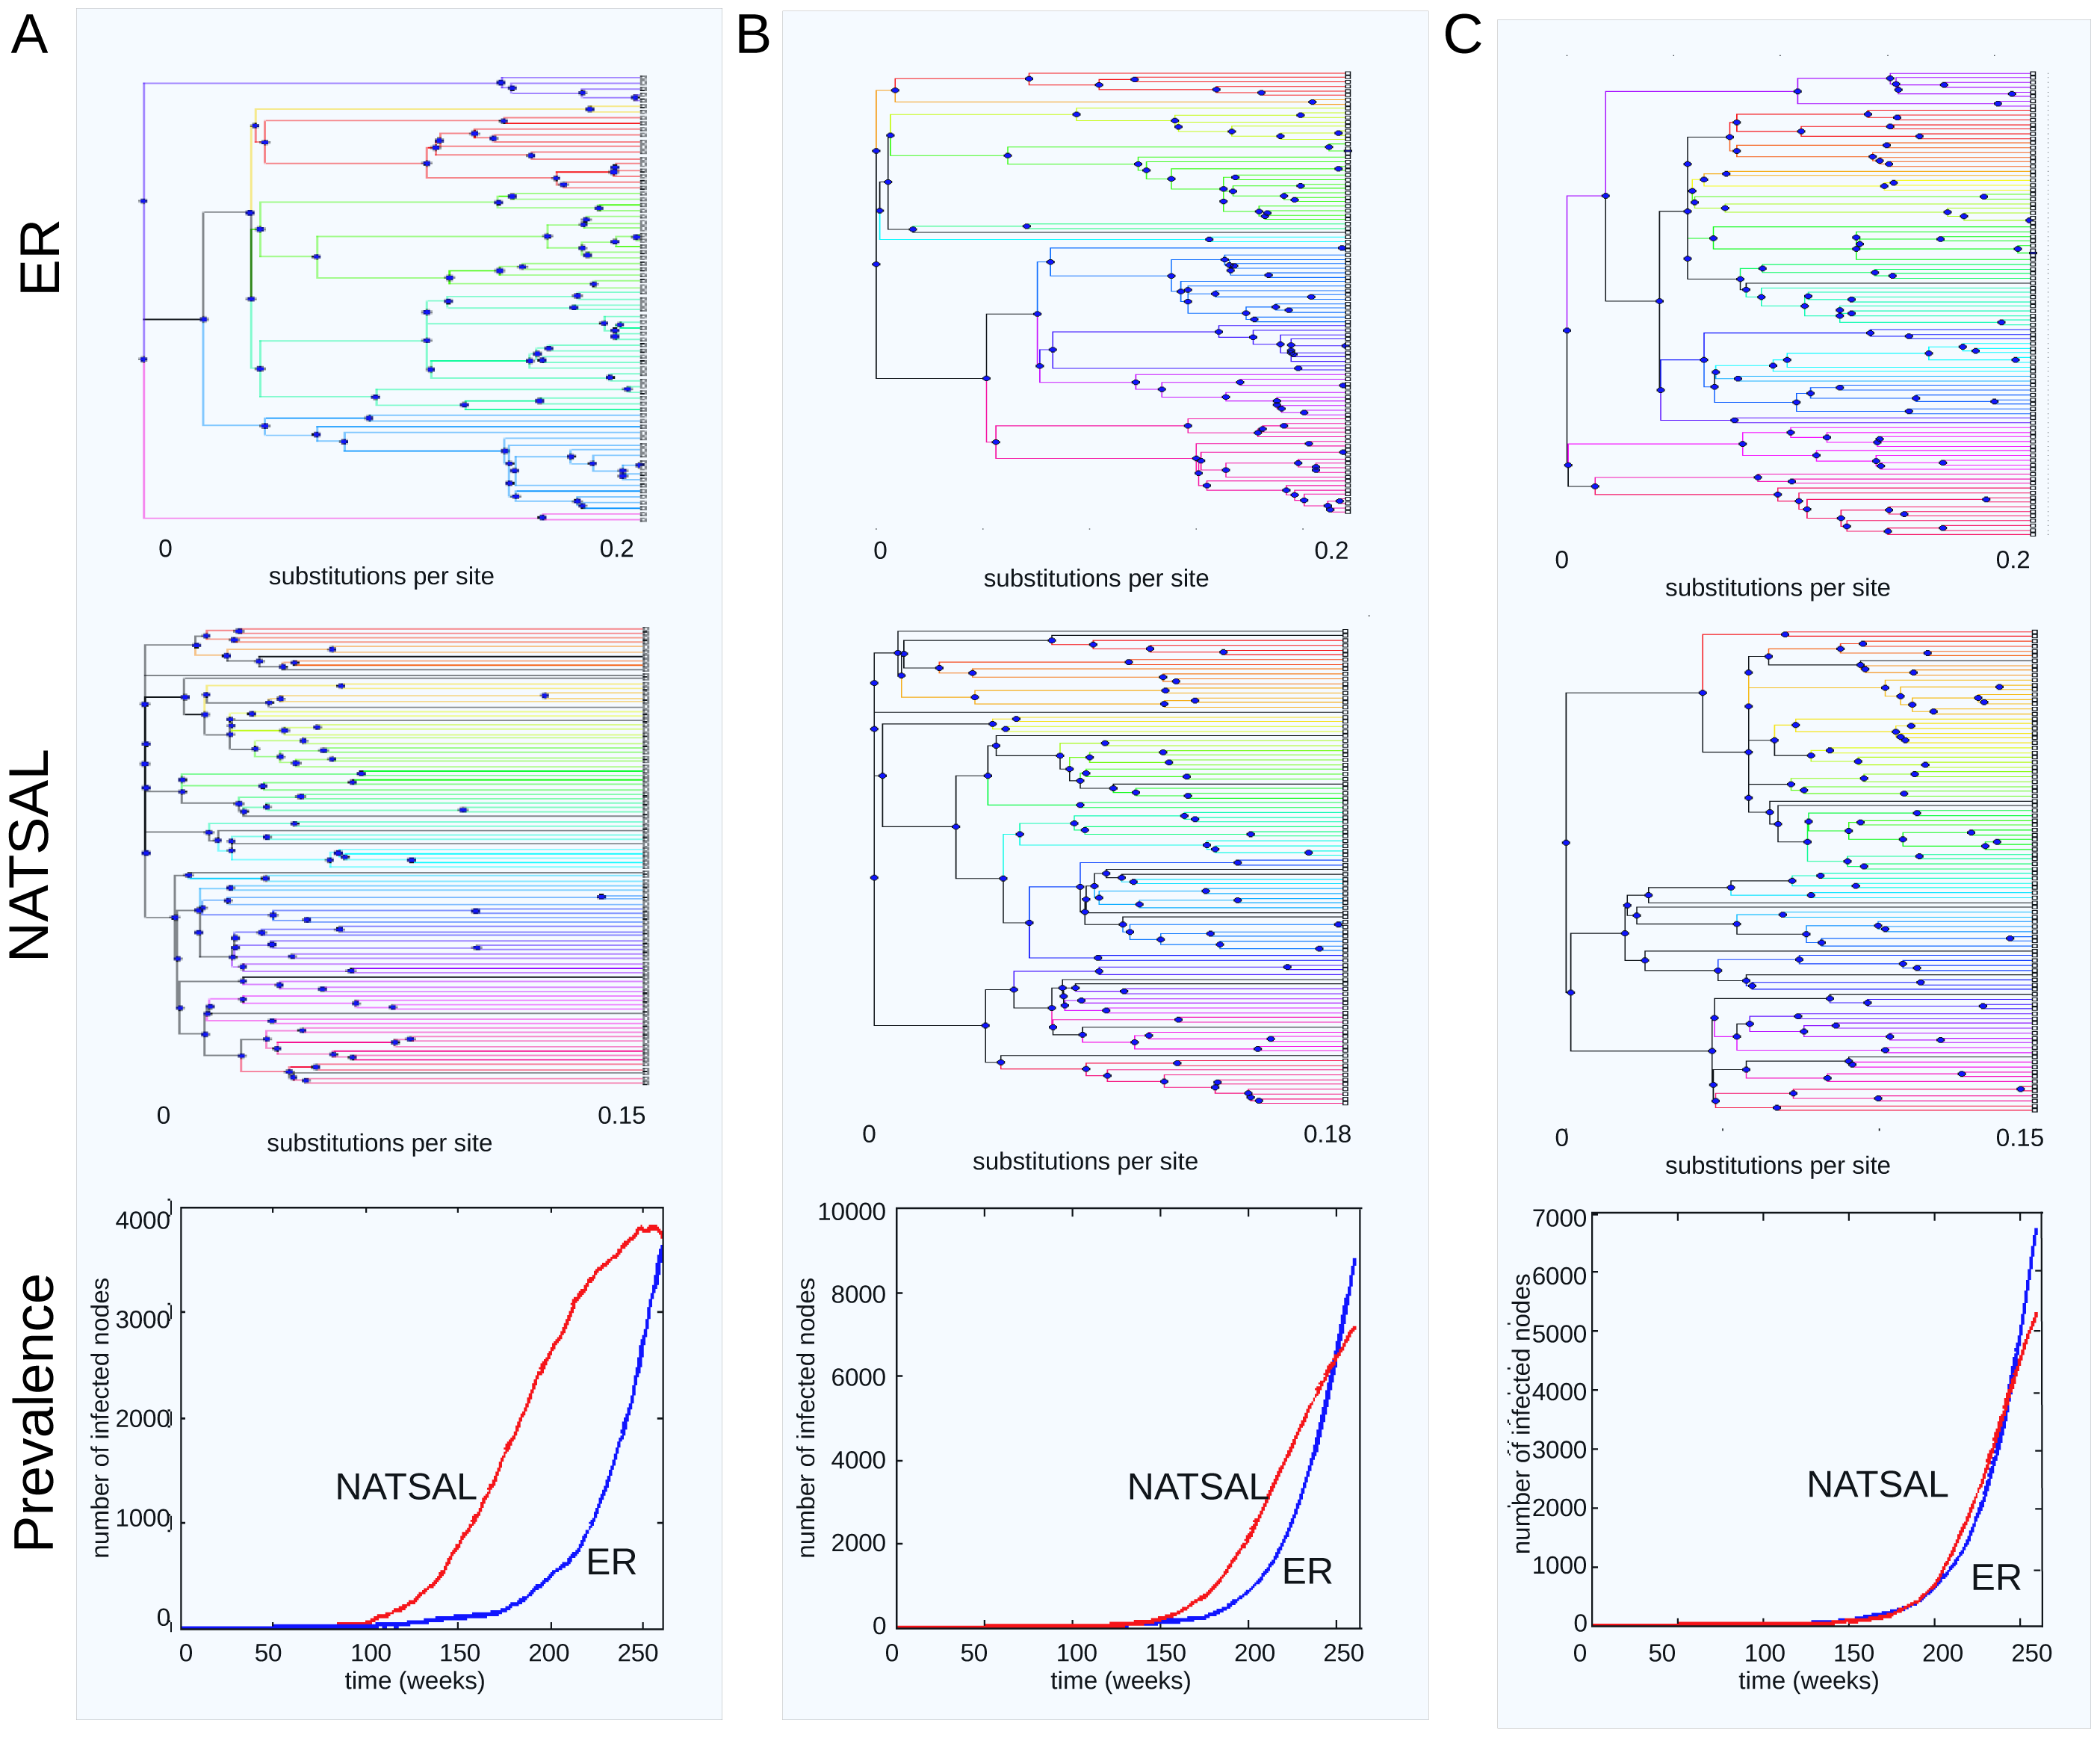
\includegraphics[height=0.8\textheight]{f4}
    \end{center}
\end{frame}

\begin{frame}{Results: degree distribution vs. cluster size distribution}
    \begin{center}
        \vspace{-0.5cm}
        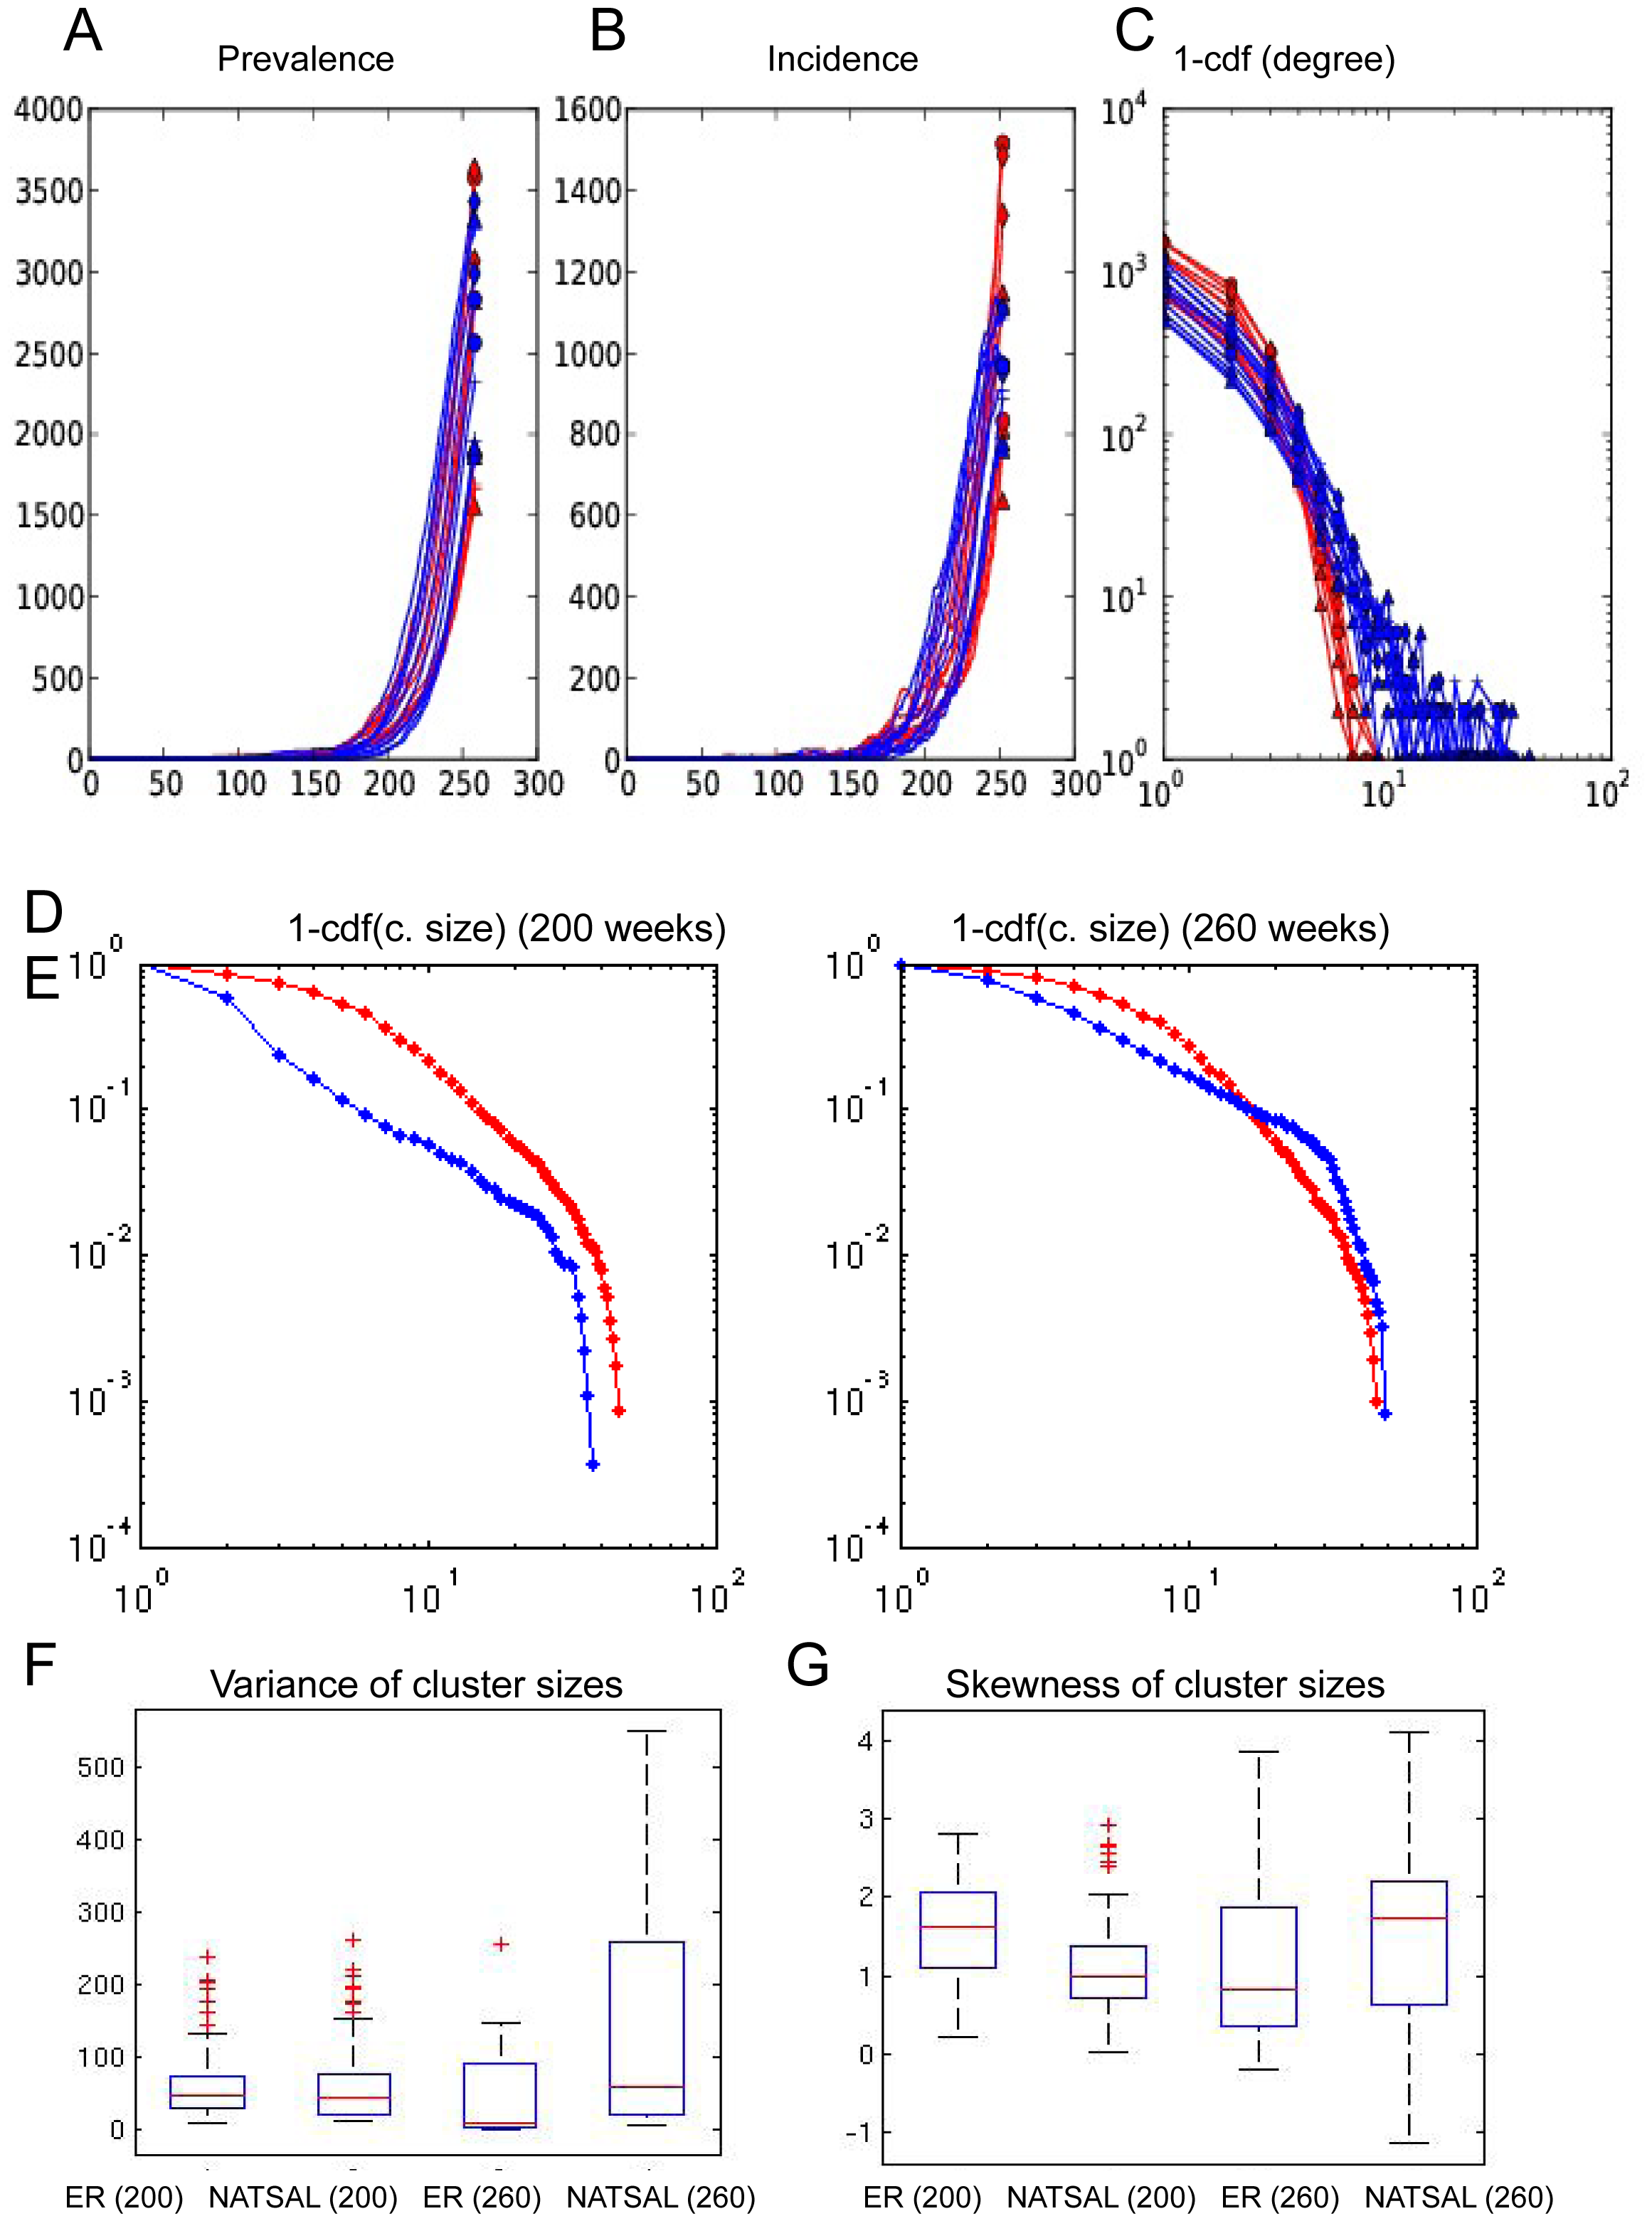
\includegraphics[width=0.7\textwidth, trim=0 2.3cm 0 0, clip=true]{f5}
    \end{center}
\end{frame}

\begin{frame}{Results: branch lengths}
    \begin{center}
        \vspace{-0.5cm}
        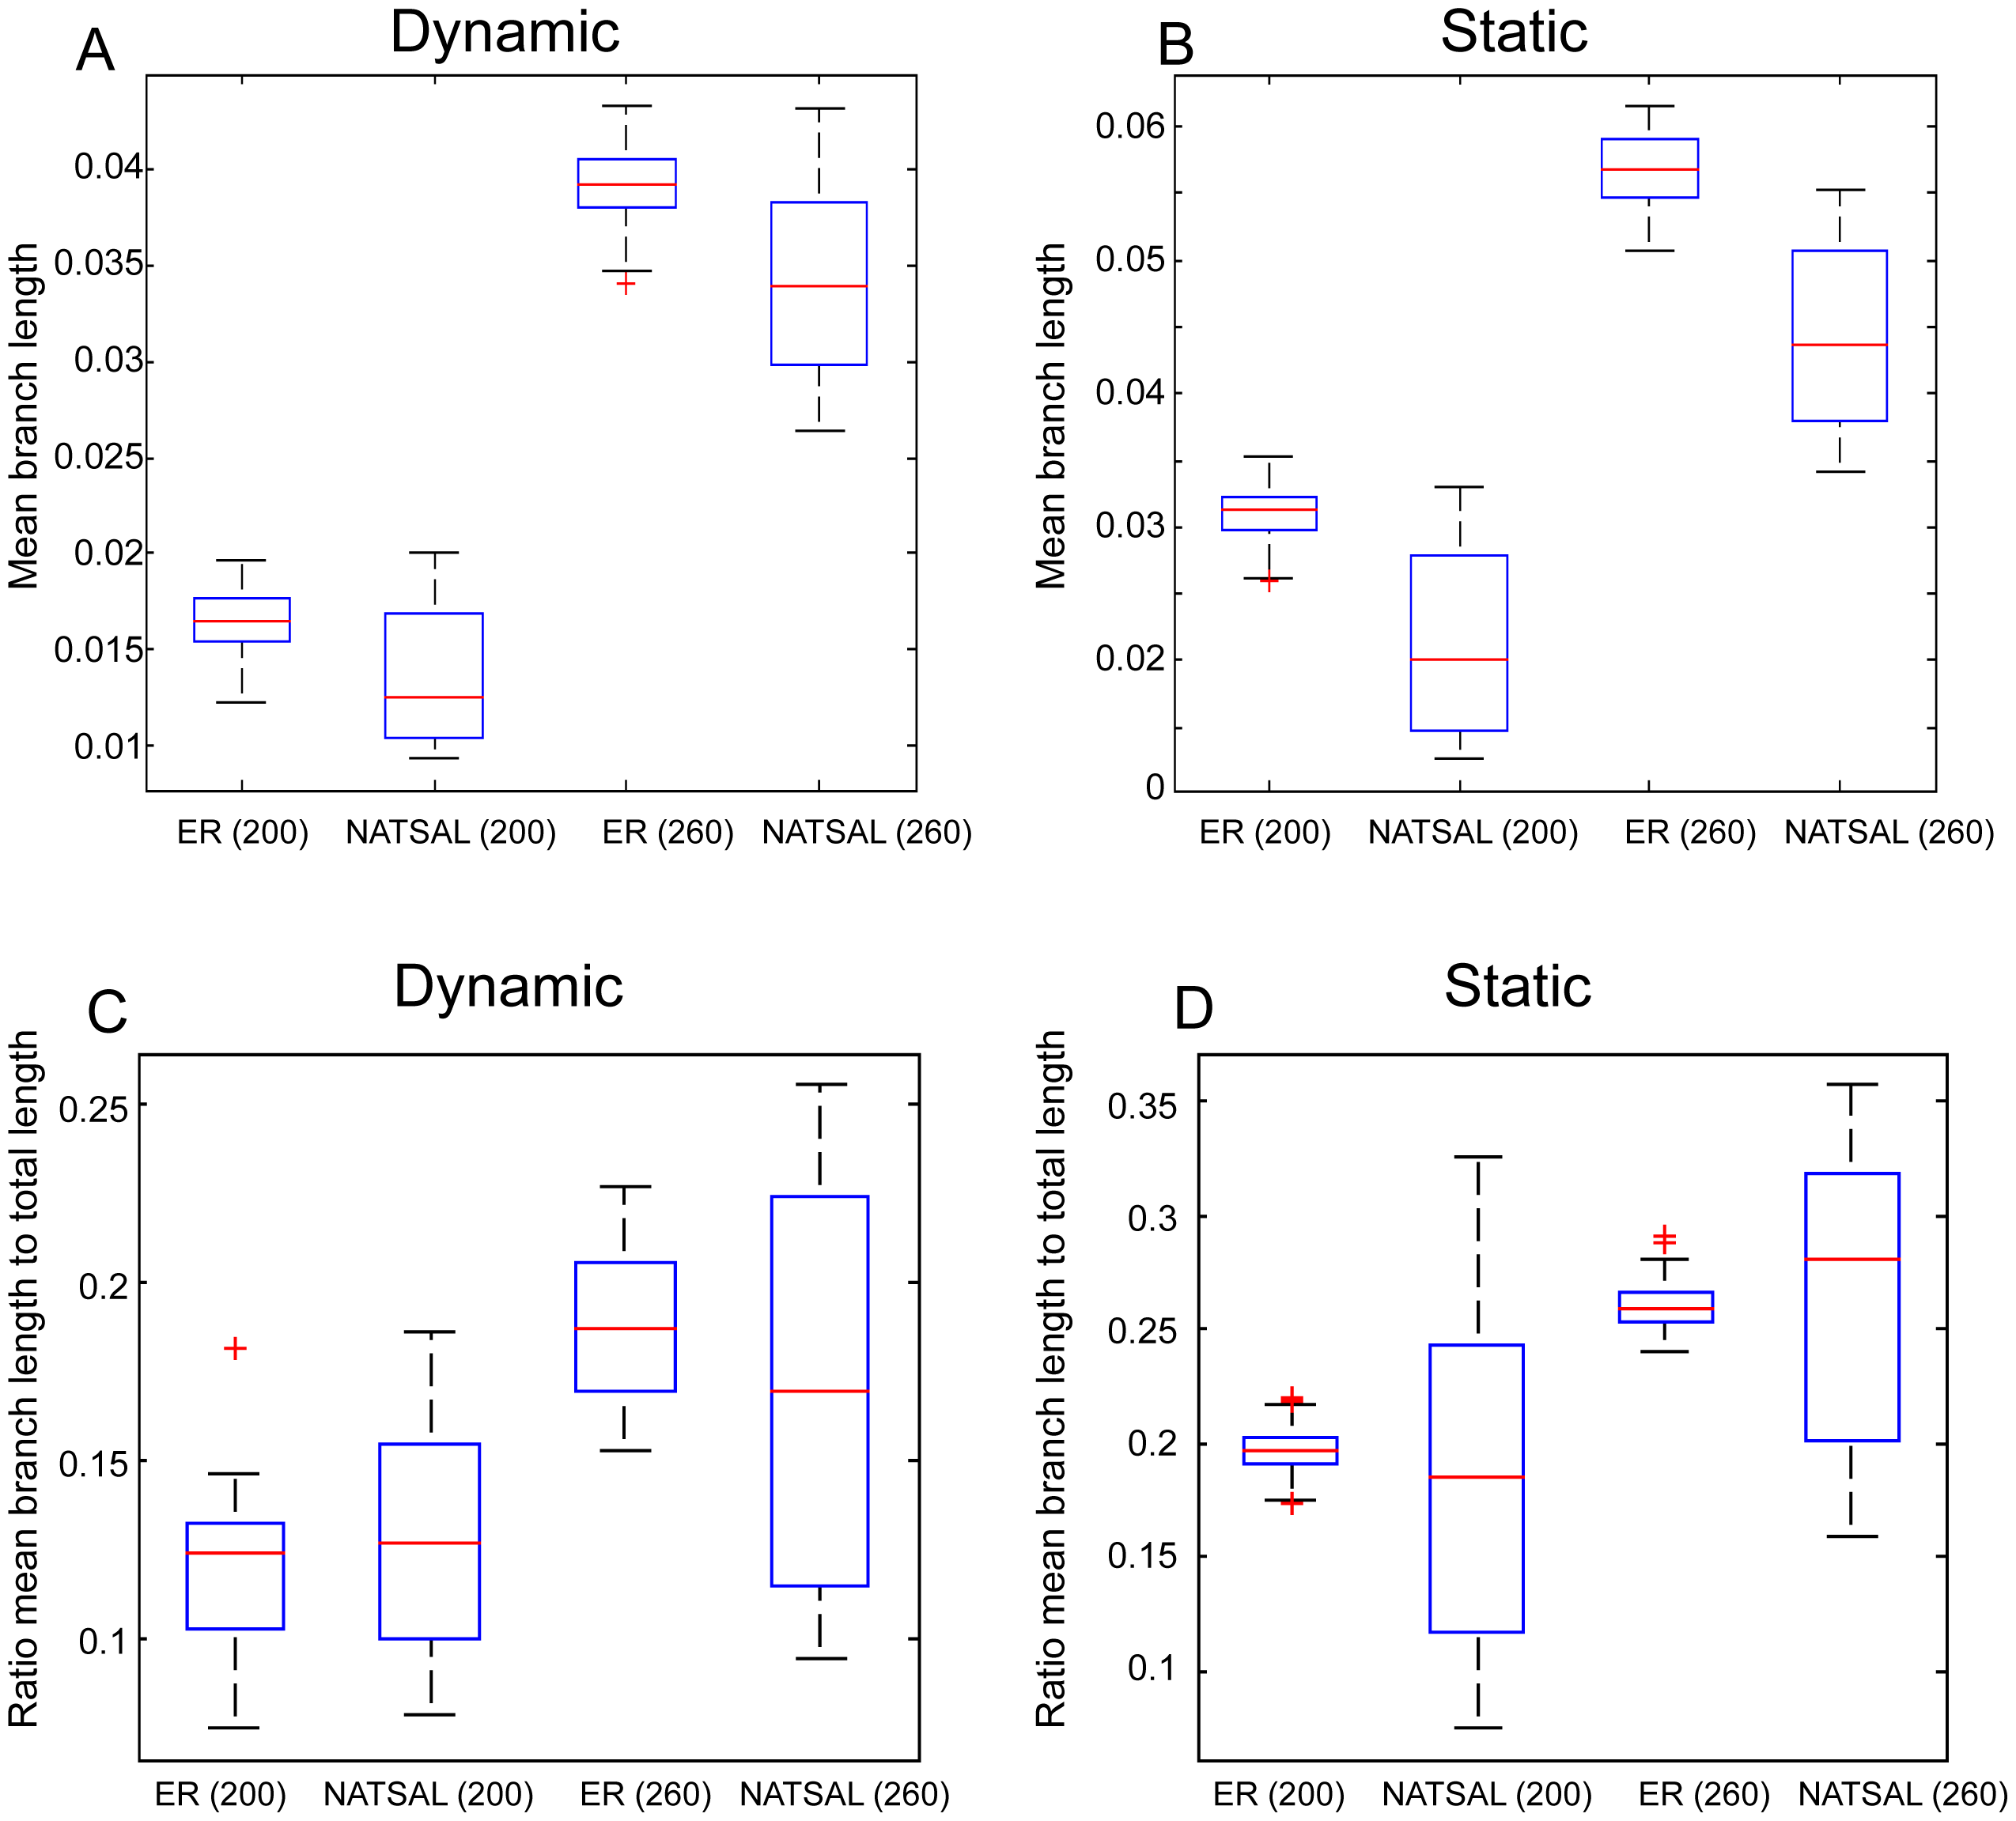
\includegraphics[height=0.8\textheight]{f6}
    \end{center}
\end{frame}

\begin{frame}{Results: star-like-ness and imbalance}
    \begin{center}
        \vspace{-0.5cm}
        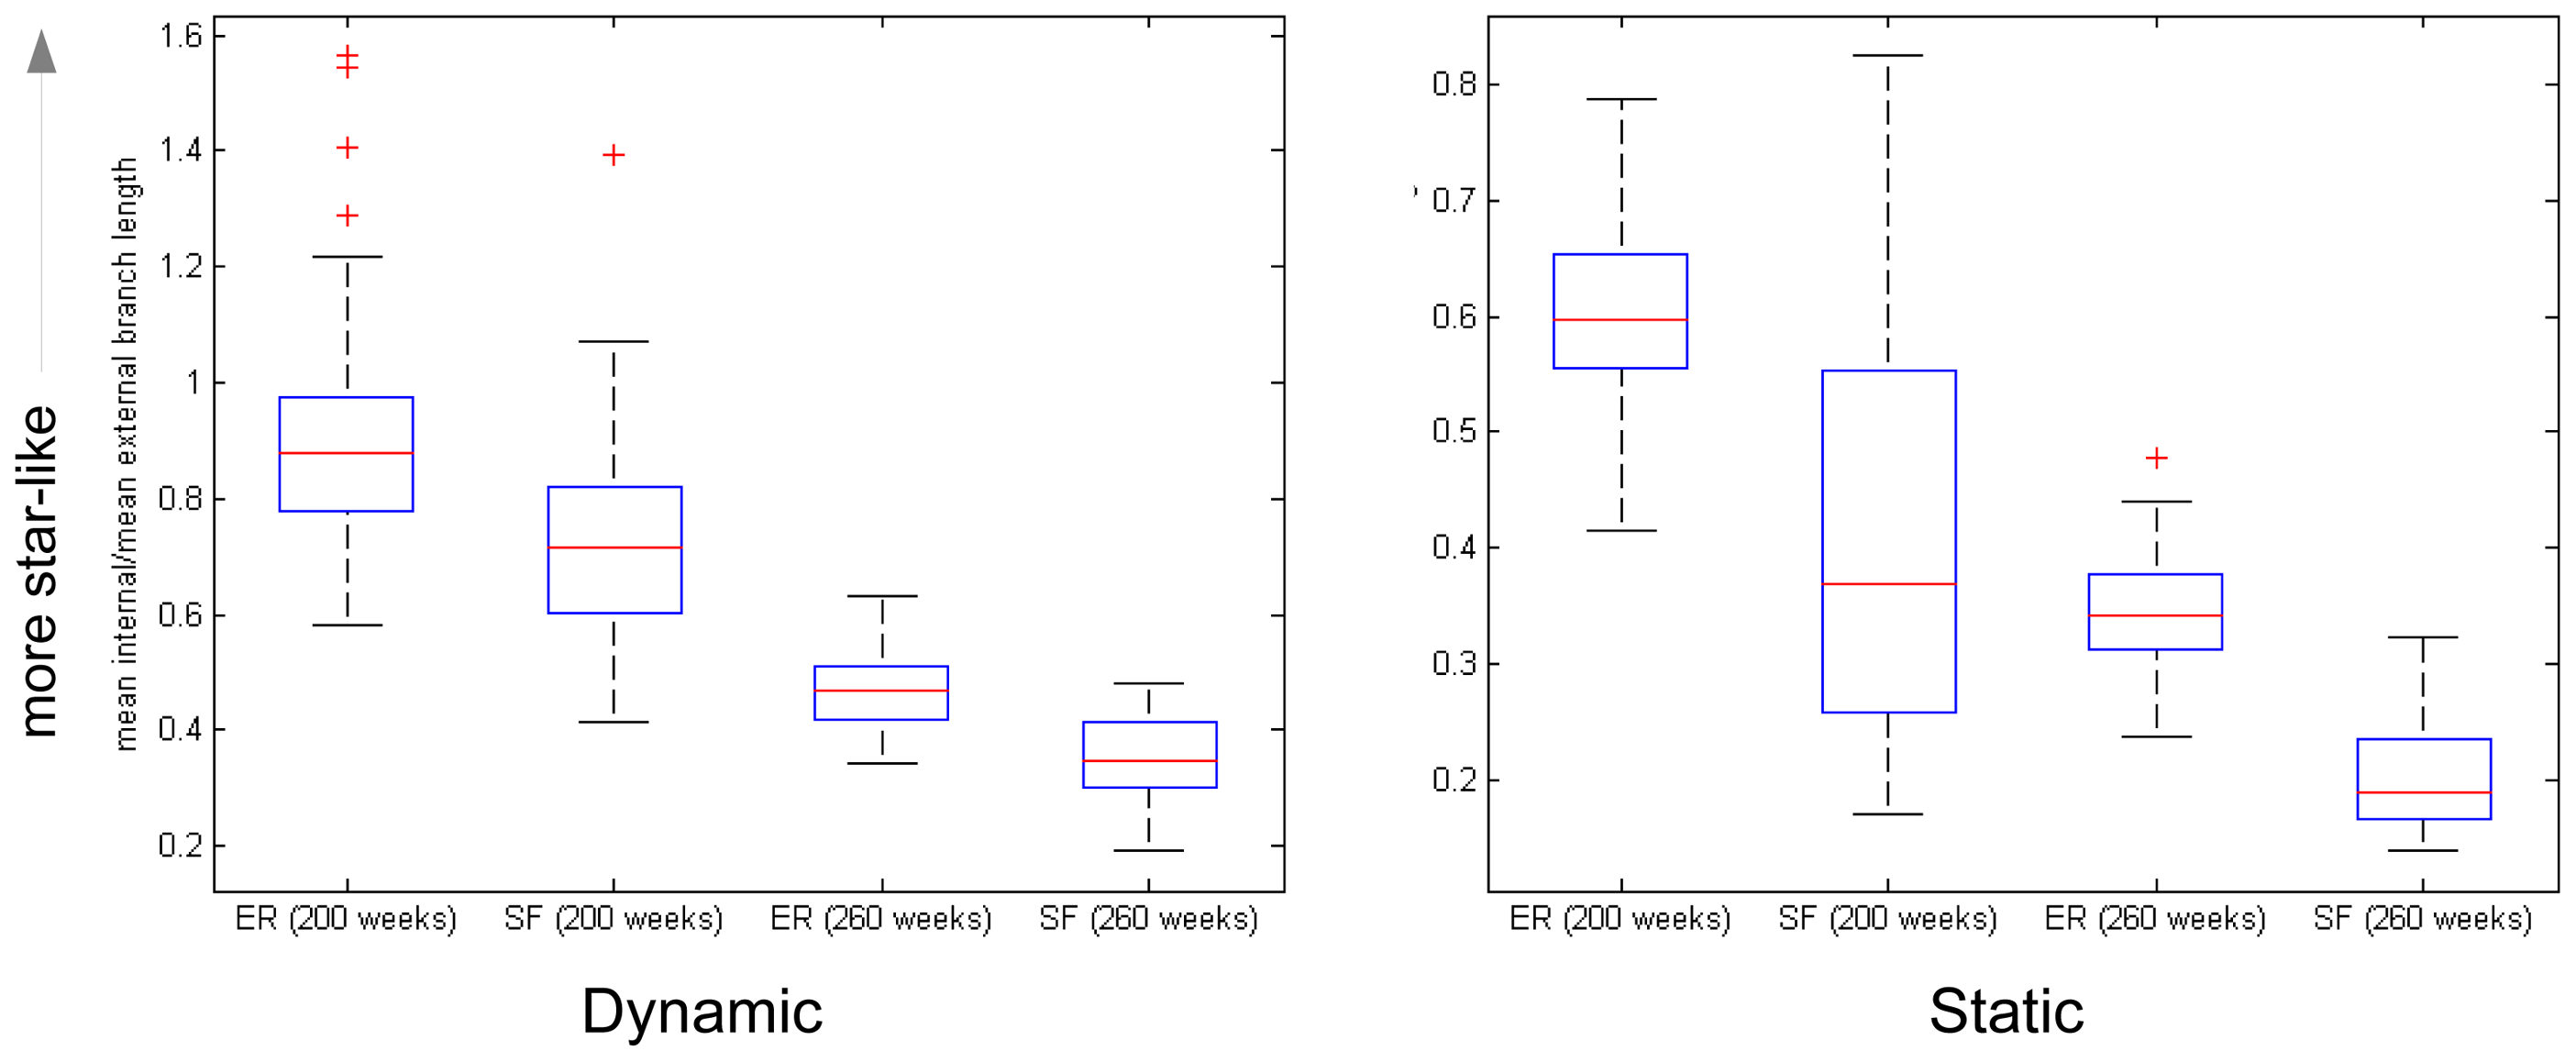
\includegraphics[width=0.8\textwidth]{f7}

        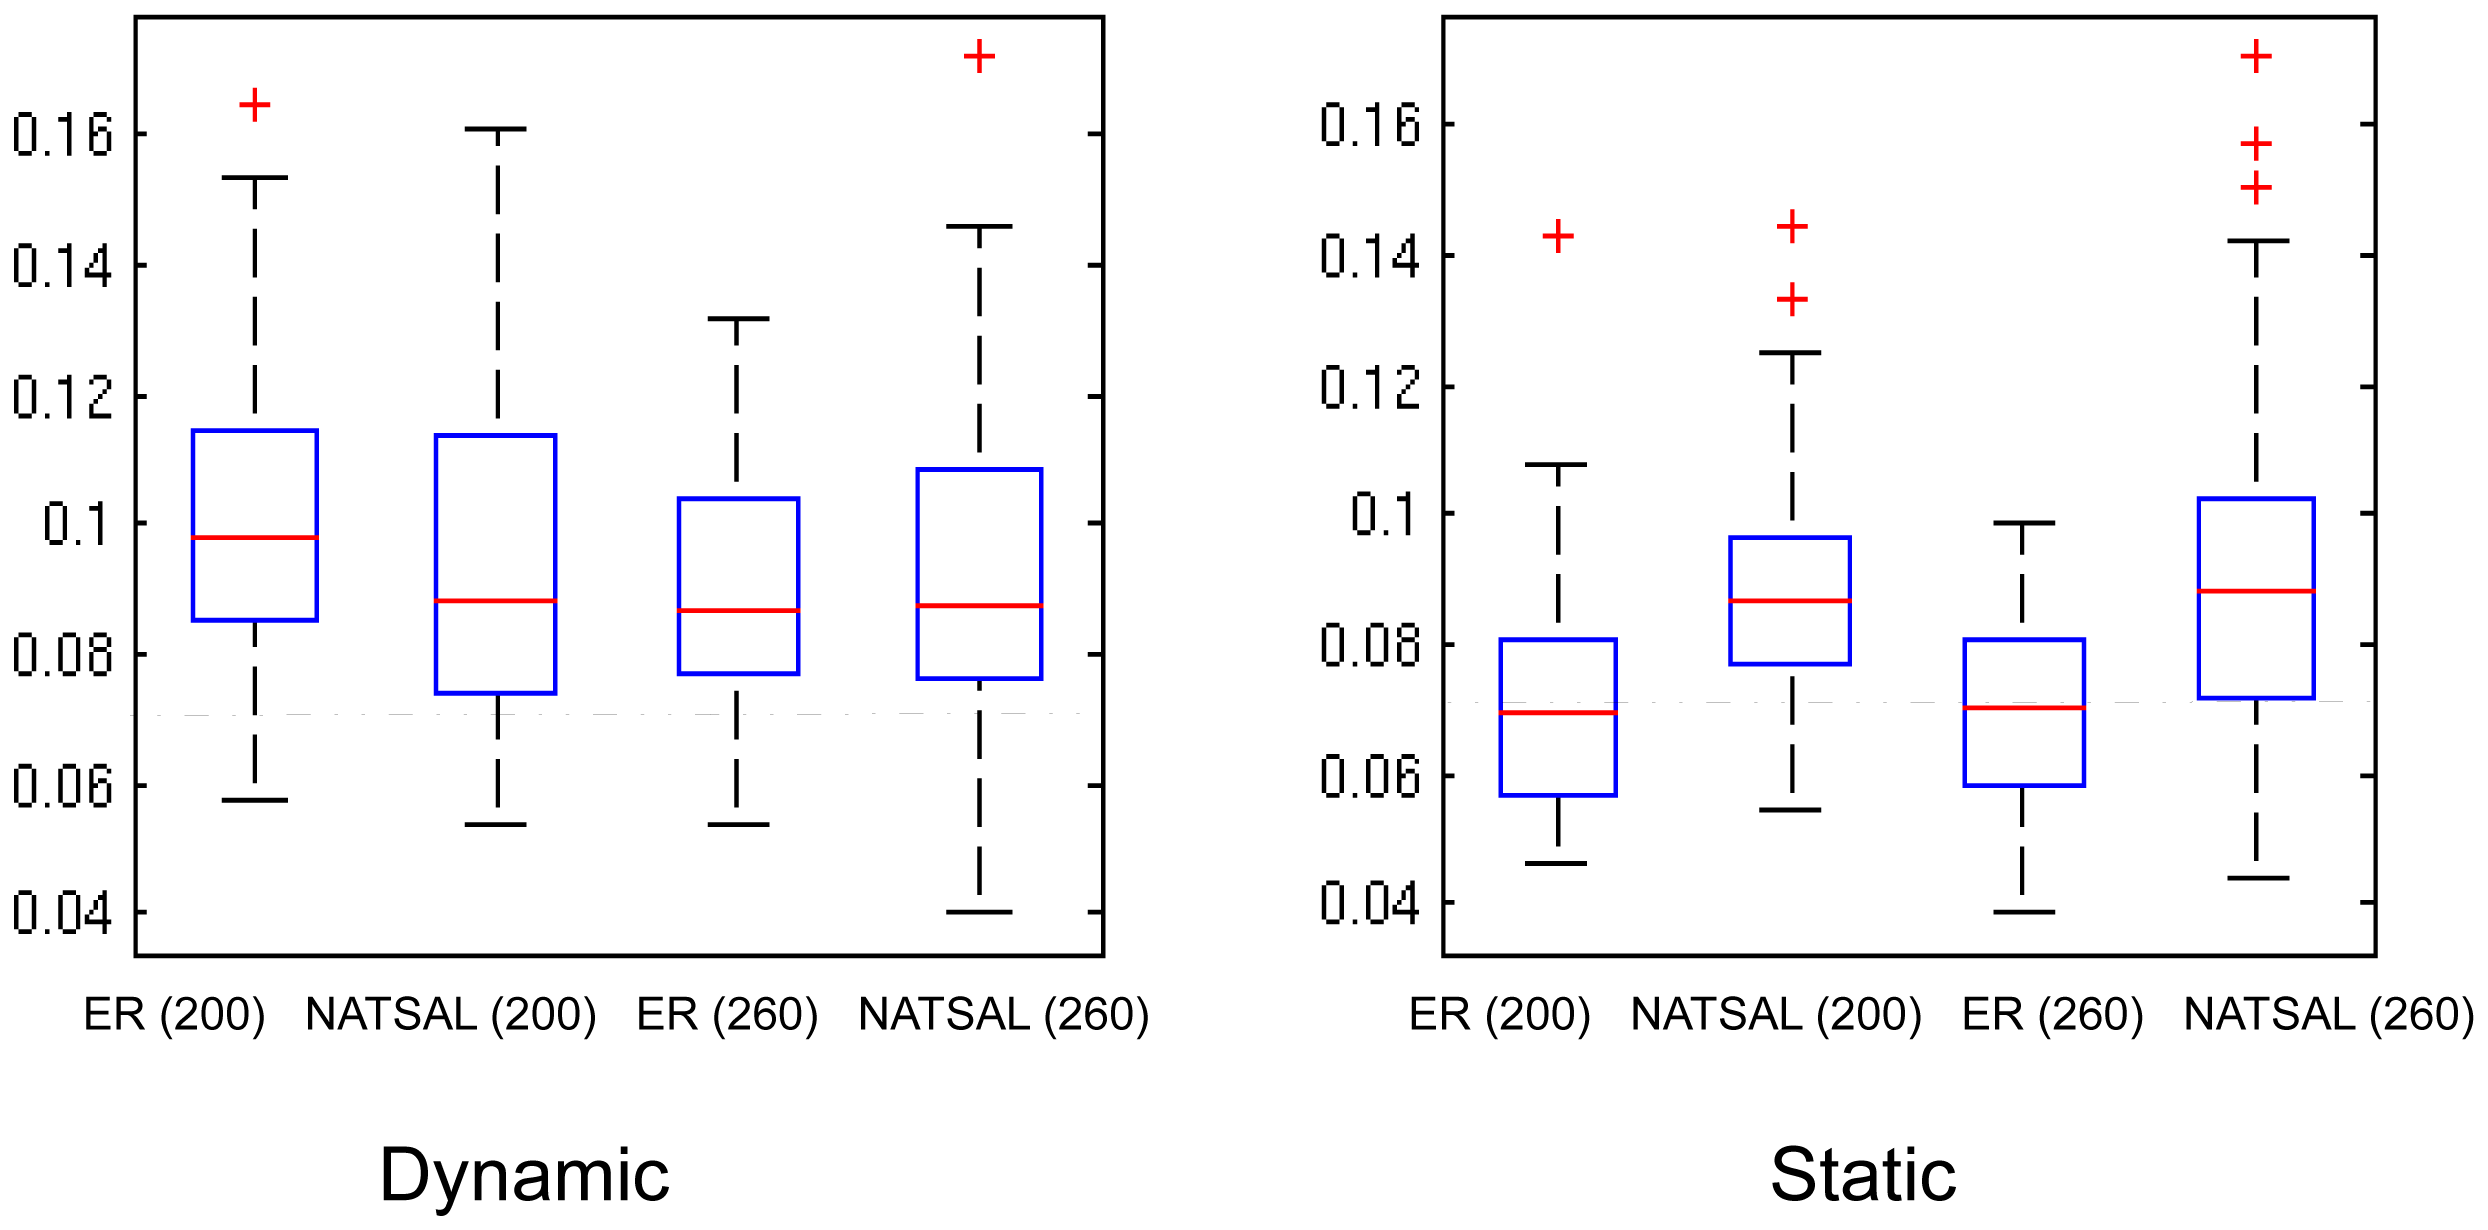
\includegraphics[width=0.7\textwidth]{f8}
    \end{center}
\end{frame}

\begin{frame}{Results: different trees from similar epidemics}
    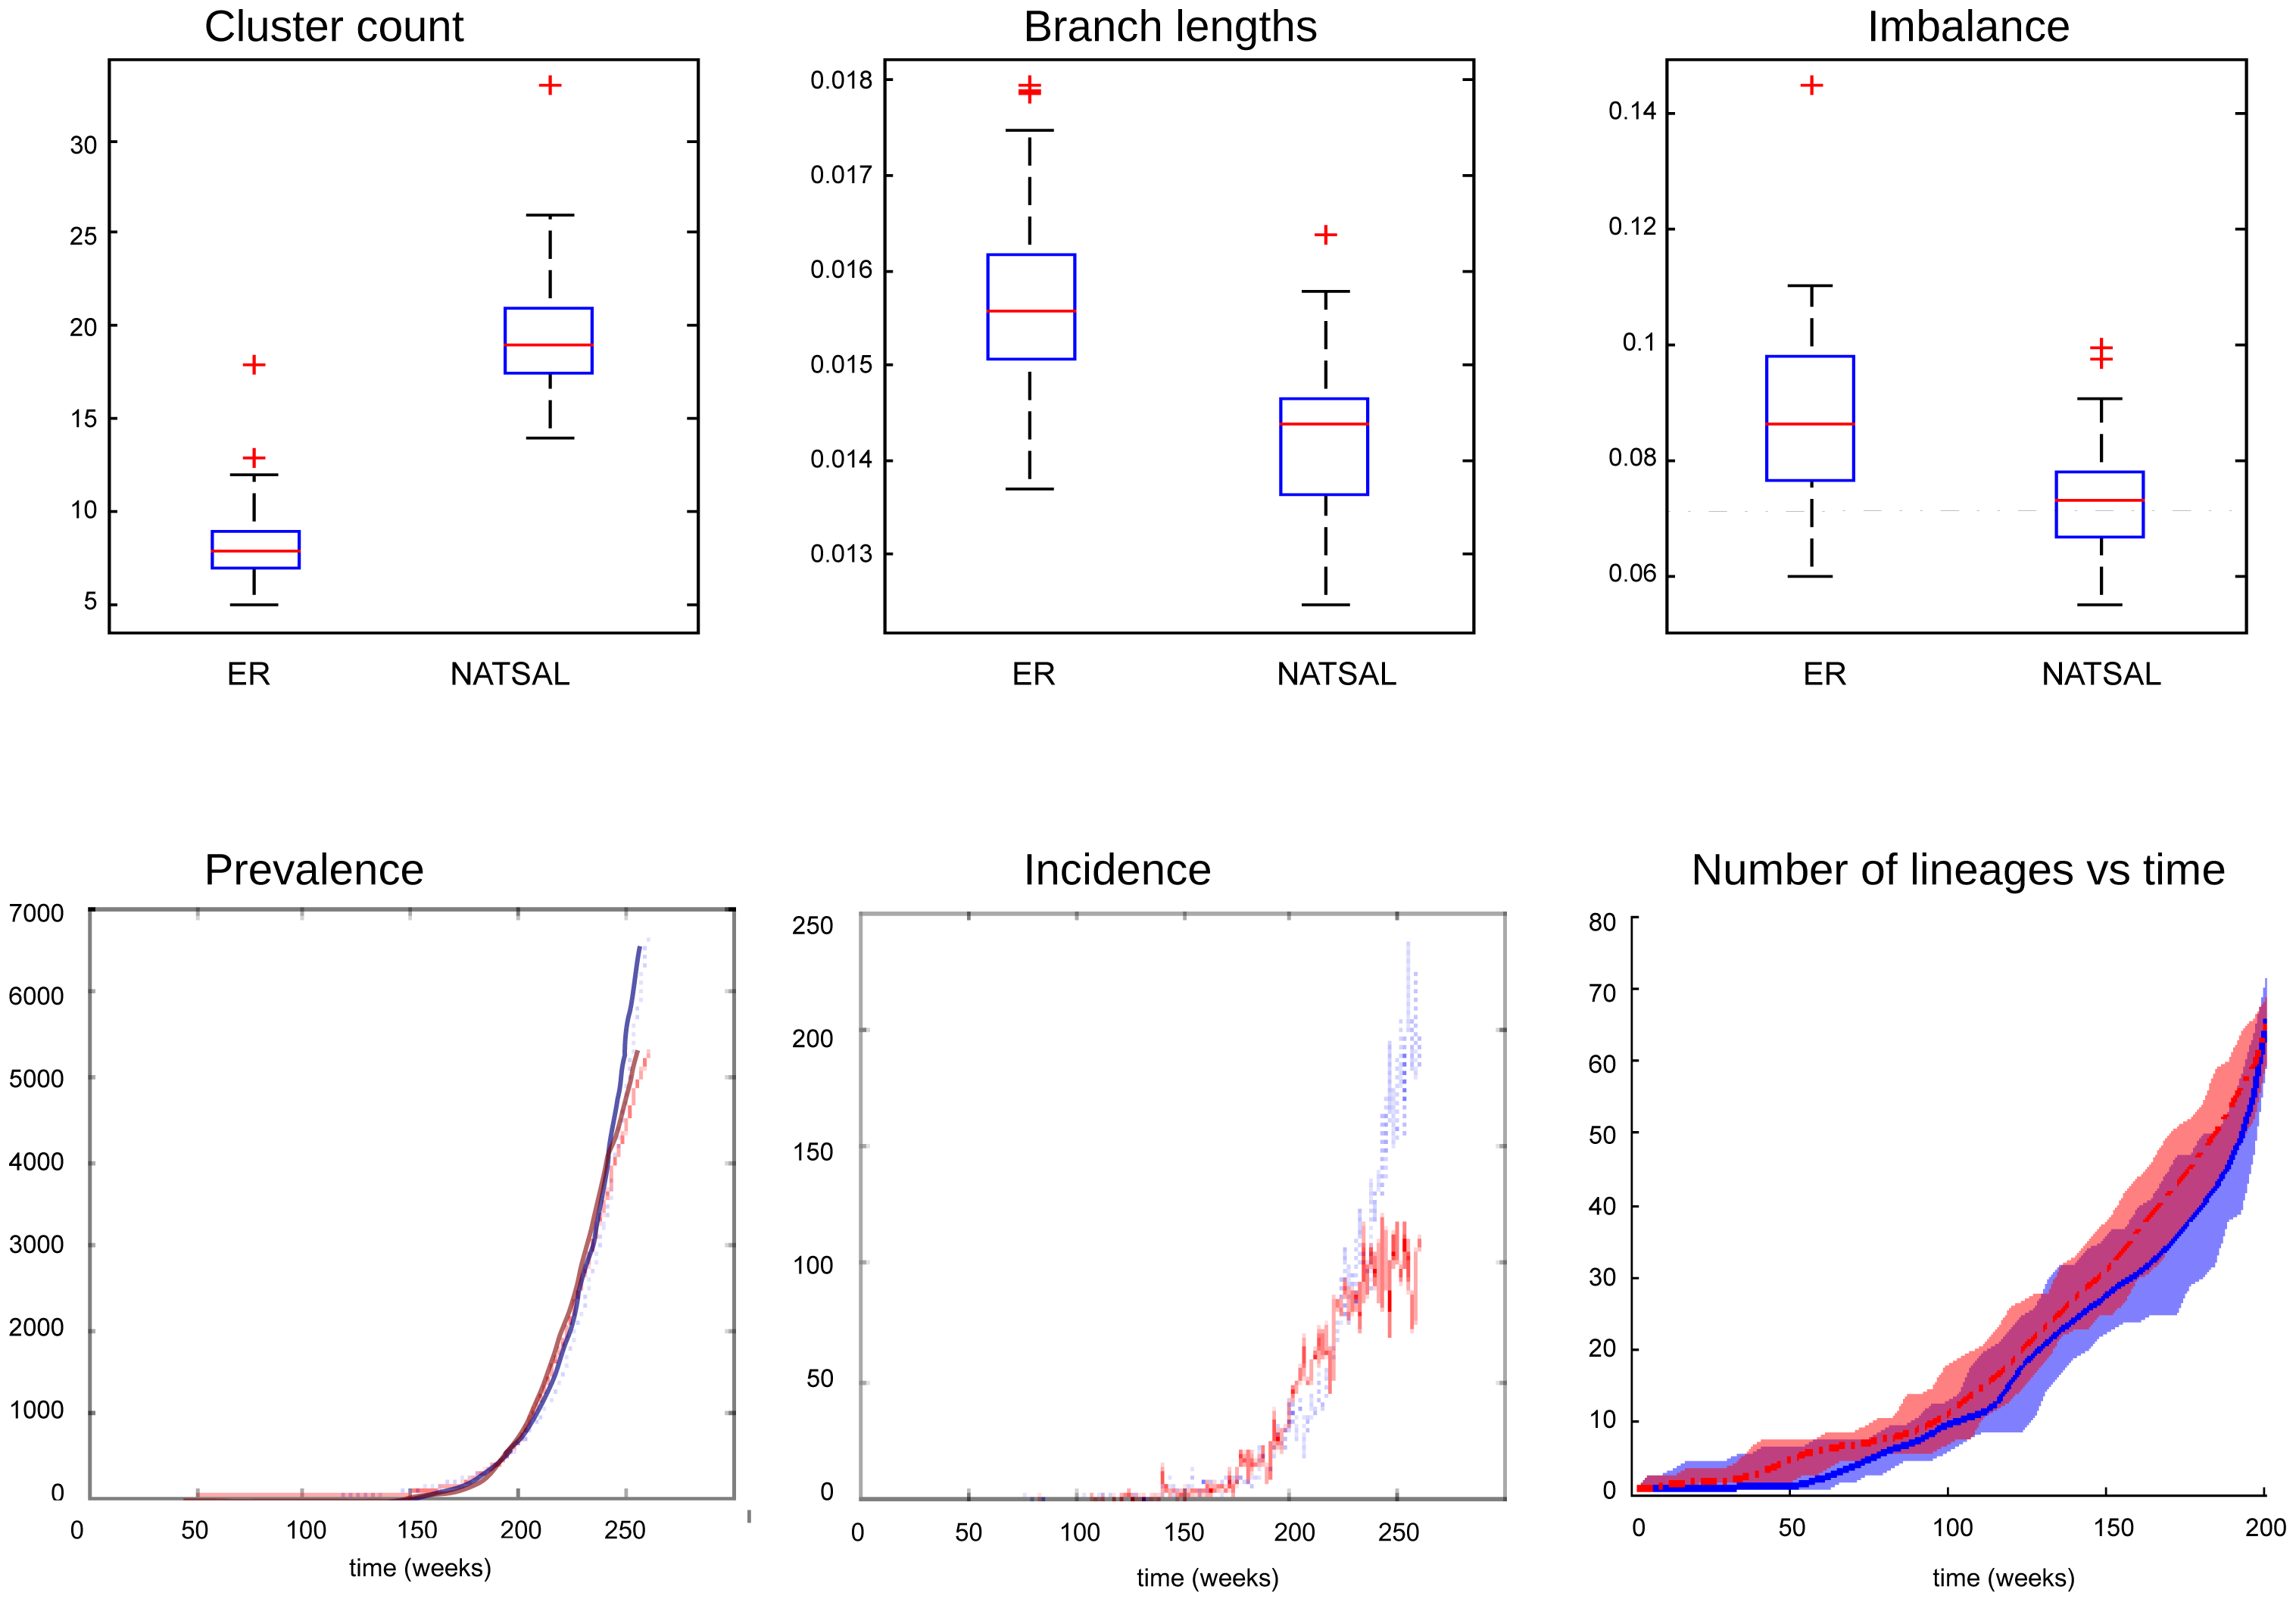
\includegraphics[width=\textwidth]{f9}
\end{frame}

\begin{frame}{Results: sampling influences imbalance and clustering}
    \begin{center}
        \vspace{-0.5cm}
        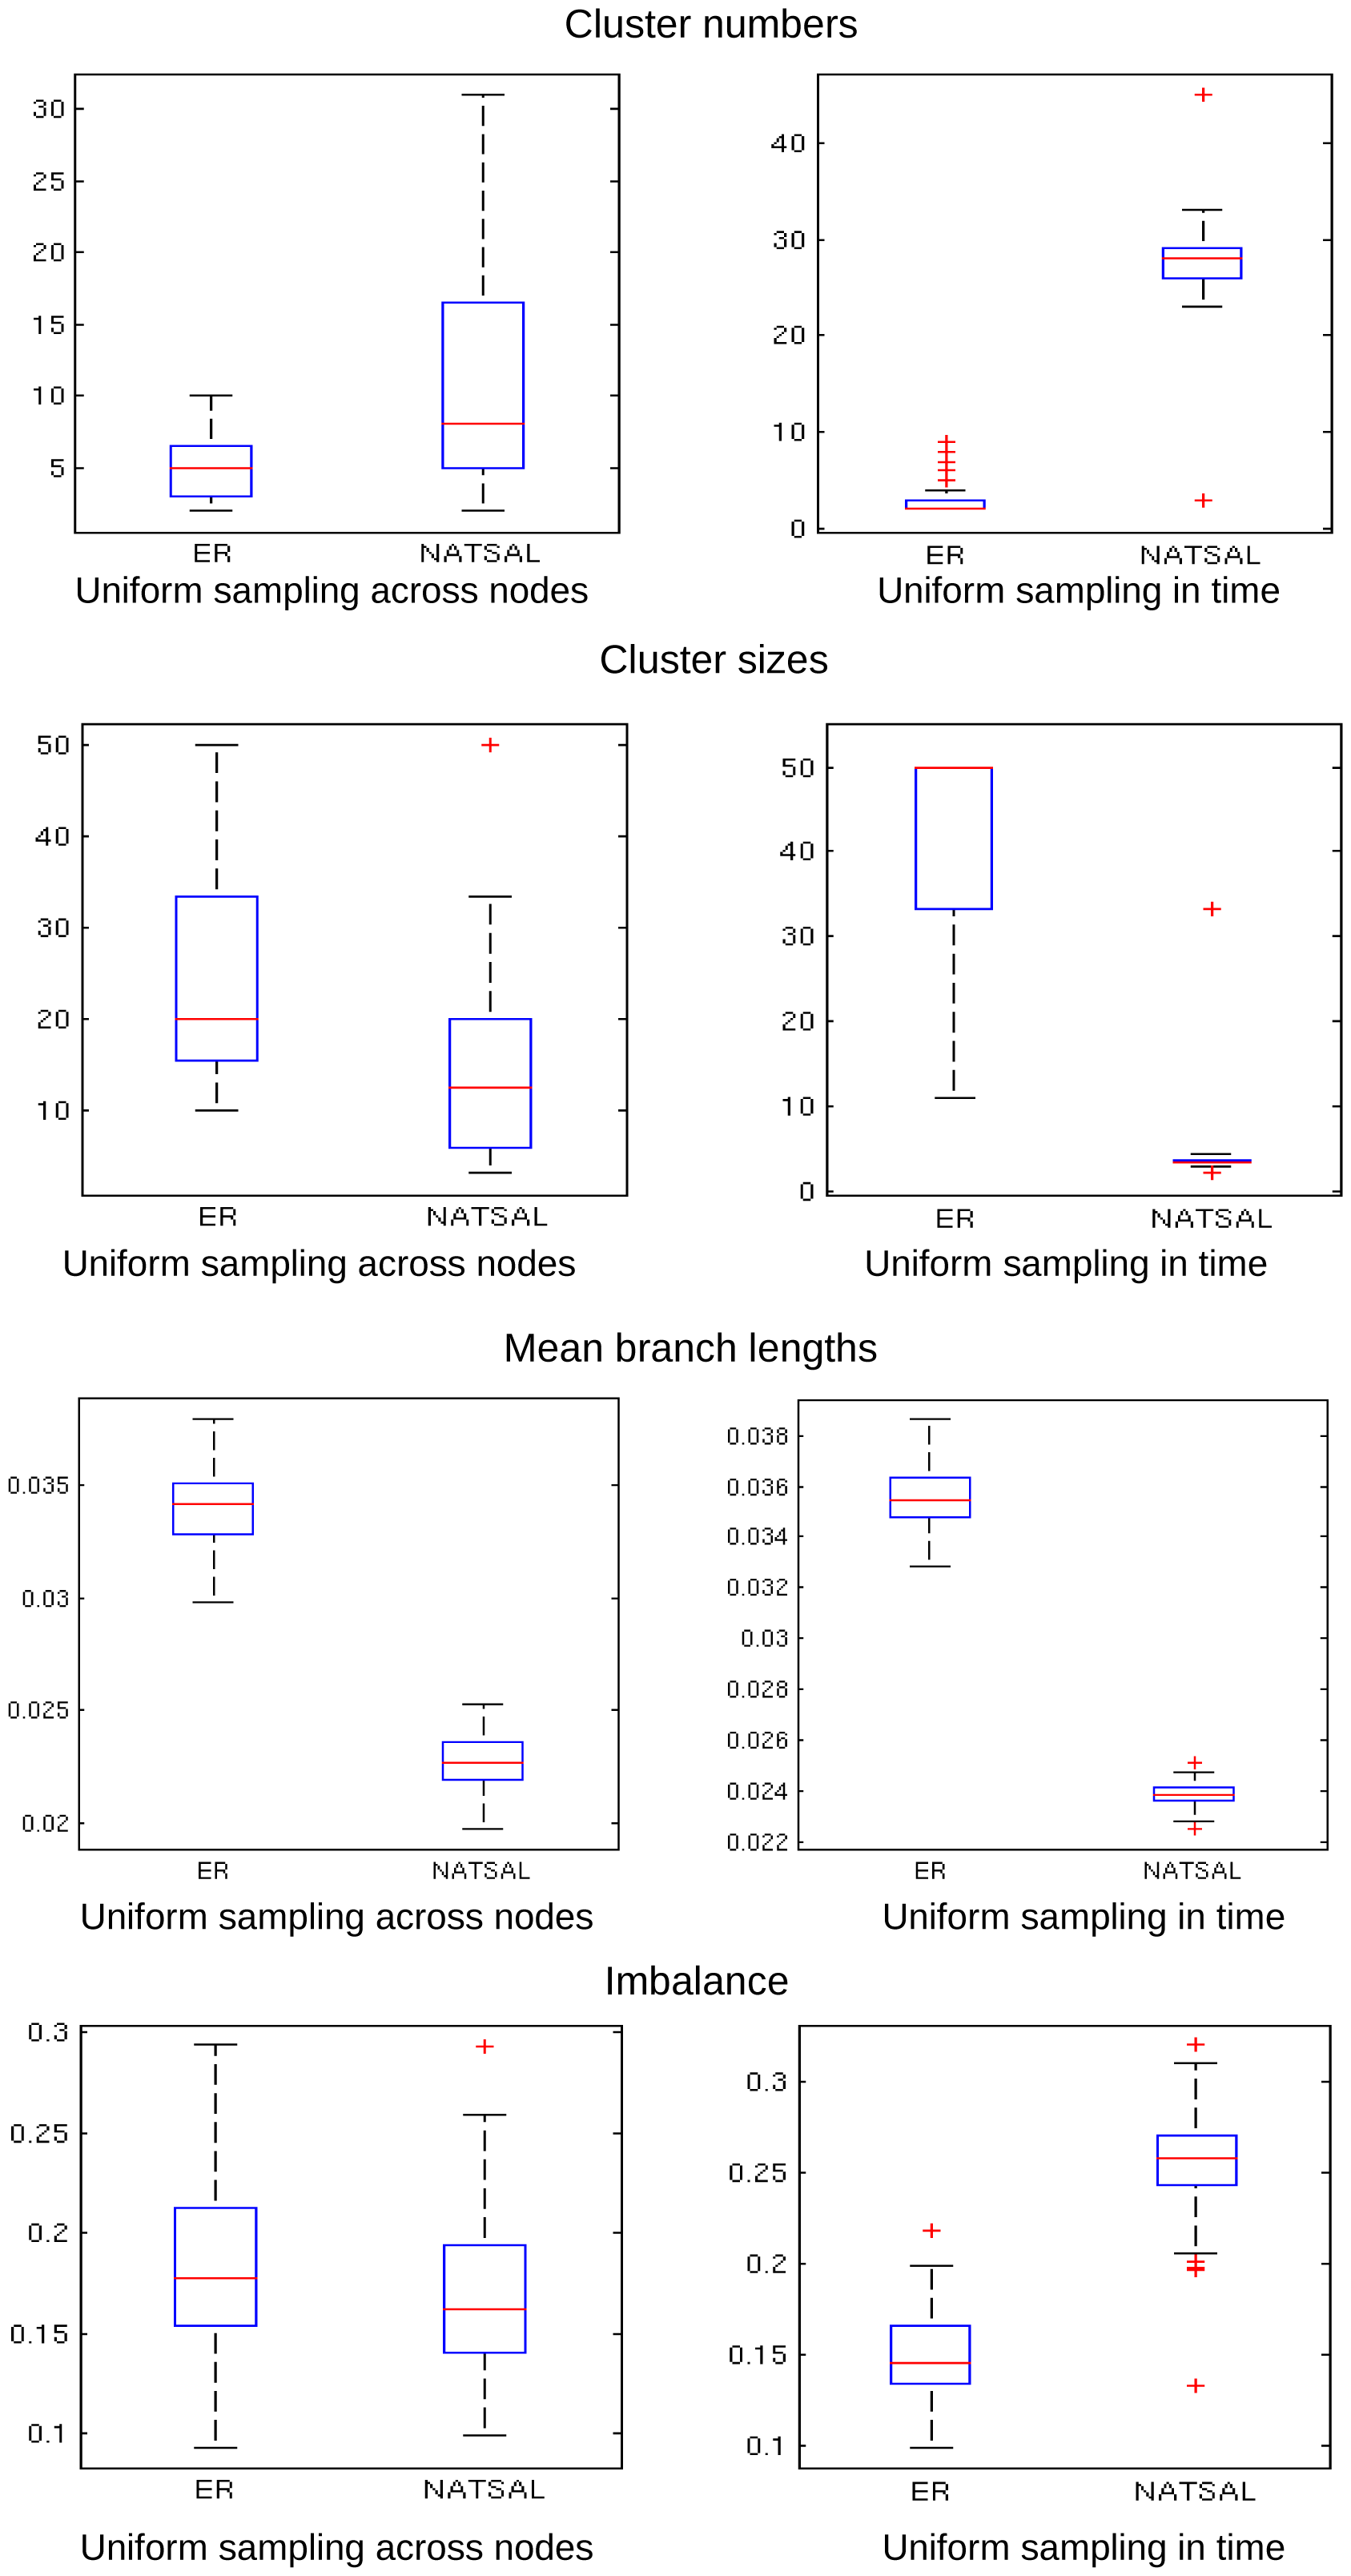
\includegraphics[width=0.8\textwidth, trim=0 7.1cm 0 0, clip=true]{f11}

        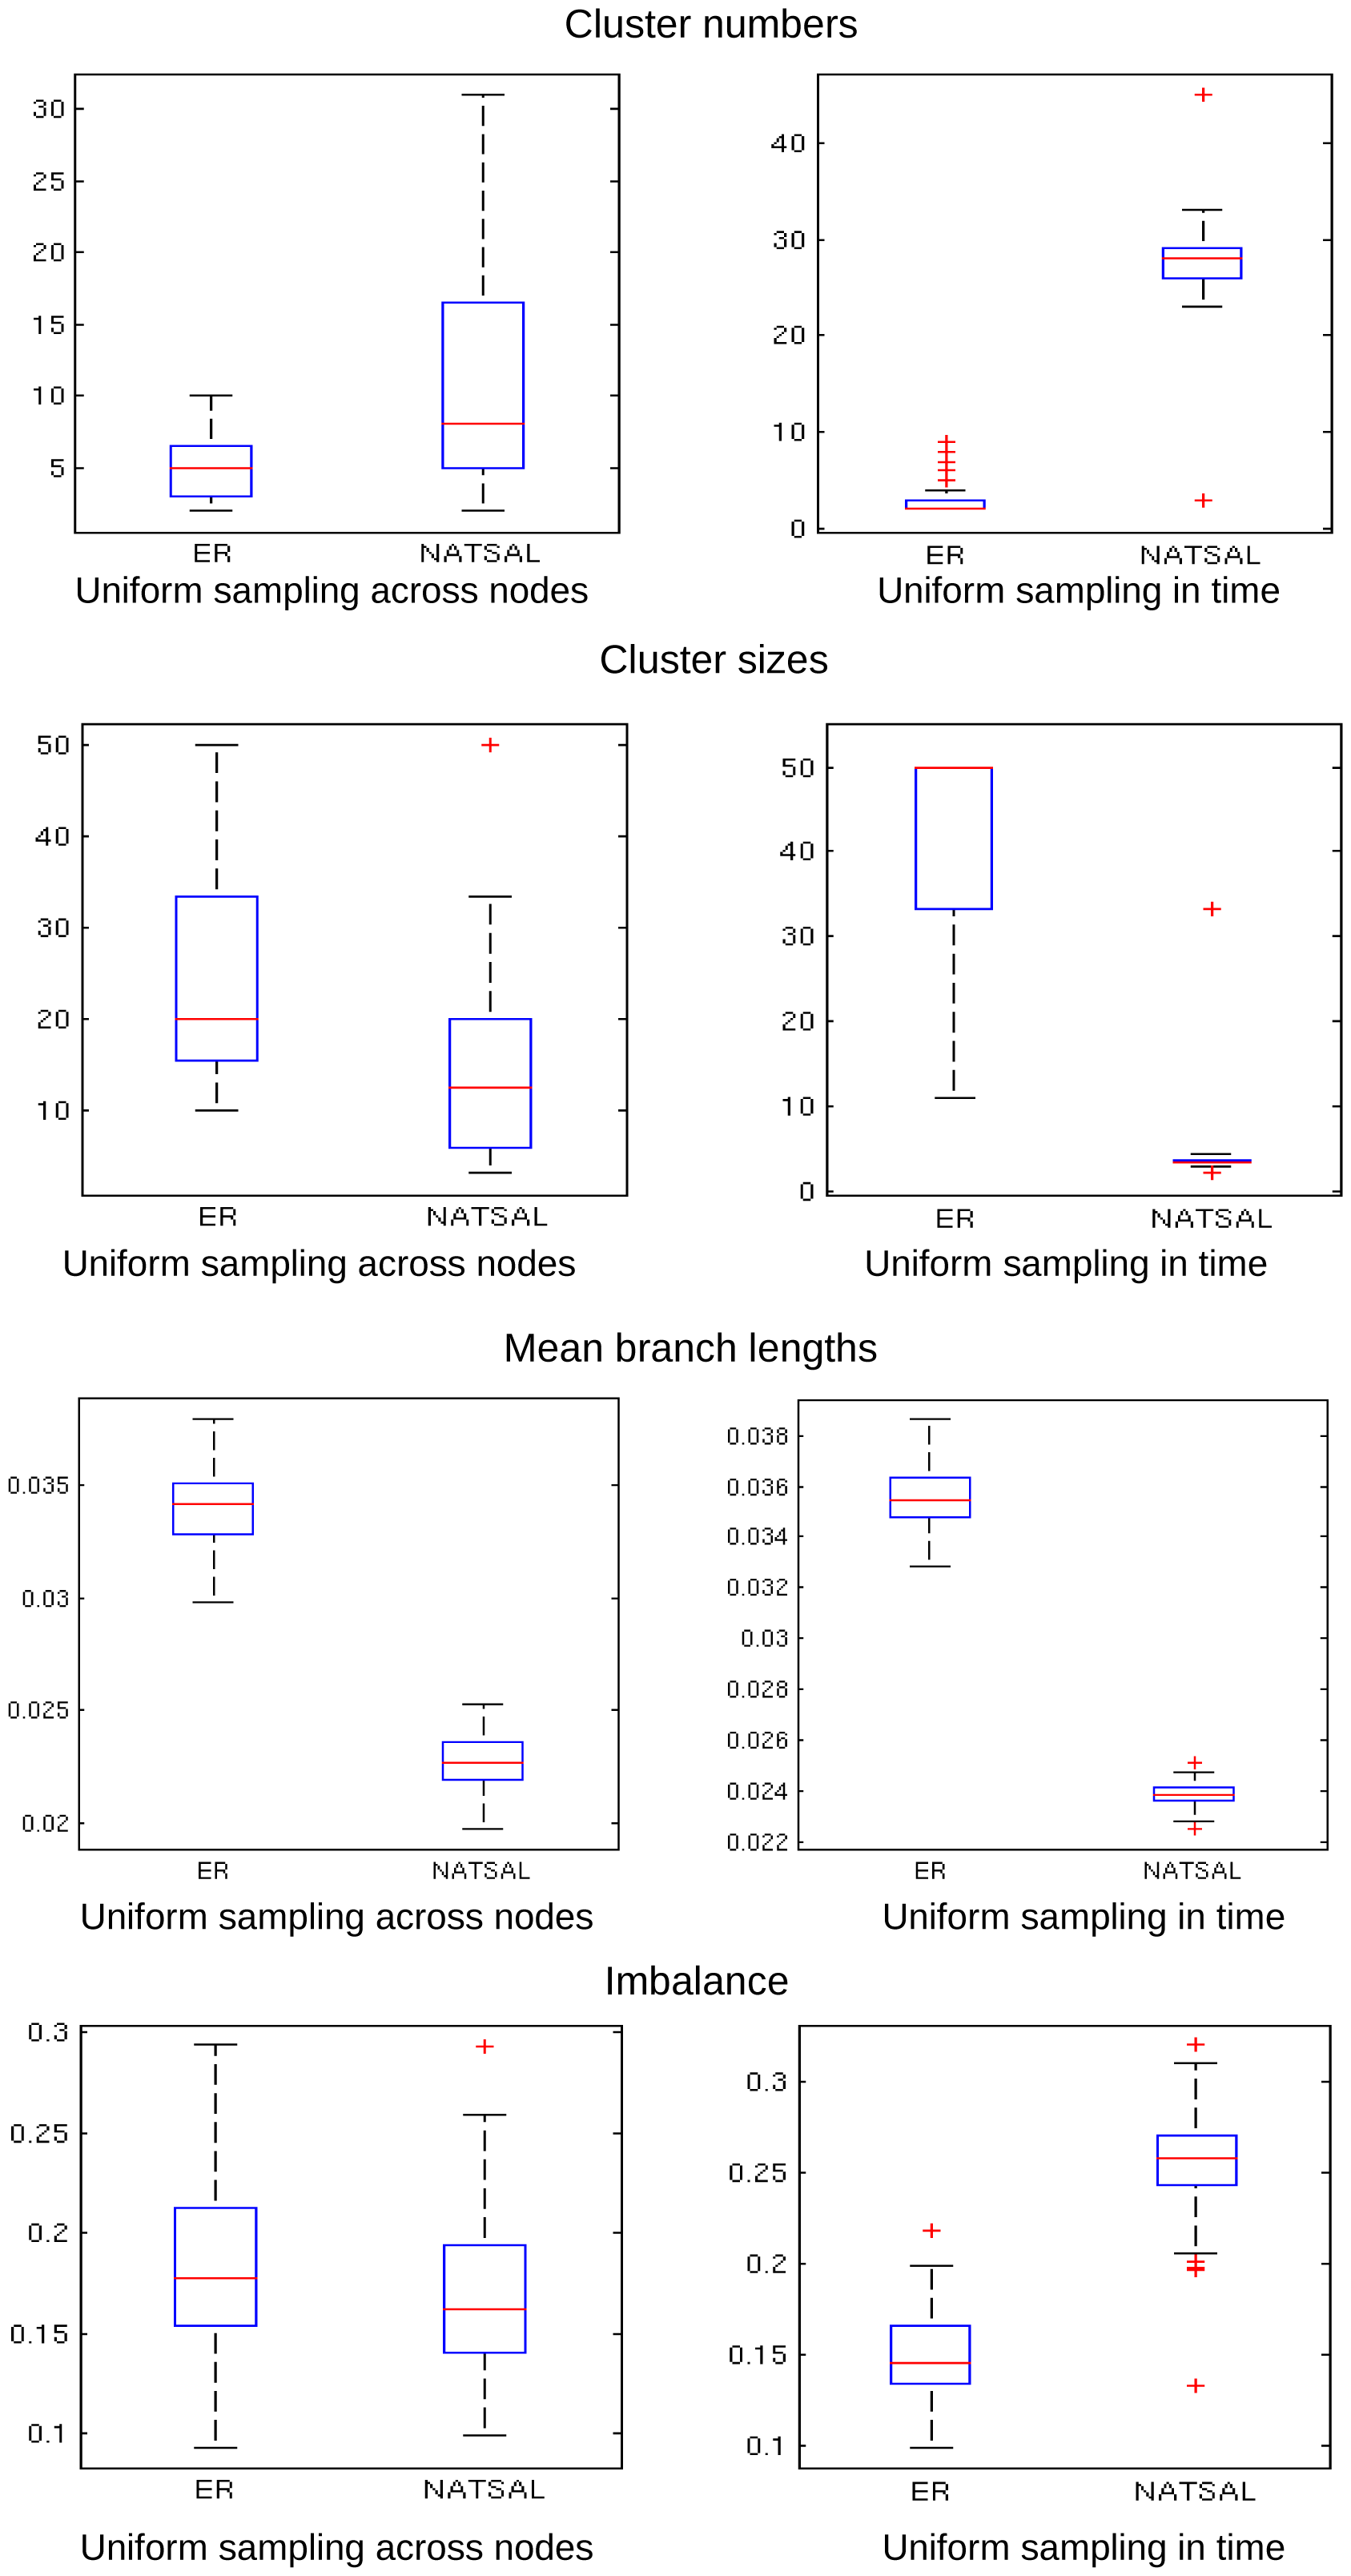
\includegraphics[width=0.8\textwidth, trim=0 0 0 6.9cm, clip=true]{f11}
    \end{center}
\end{frame}

\end{document}
